\documentclass[journal]{IEEEtran}
\usepackage{amsmath,amsfonts}
\usepackage{array}
\usepackage[caption=false,font=normalsize,labelfont=sf,textfont=sf]{subfig}
\usepackage{textcomp}
\usepackage{stfloats}
\usepackage{url}
\usepackage{xurl}
\usepackage{graphicx}
\usepackage{cite}
\usepackage{tabularx}
\usepackage{booktabs}
\usepackage{float}

\graphicspath{{figures/}}

\hyphenation{op-tical net-works semi-conduc-tor IEEE-Xplore}

% NOTE: The section structure follows the CS4486 mini-project template, but the
% content is the CS4480/CS4880 Open Project (EUR-based exchange rates and
% parallel rolling correlations). Replace the course code, team name, member
% names and student IDs before submission.

\begin{document}

\title{Co-Movement, Volatility and Parallel Rolling Correlations in EUR-Based Exchange Rates}

\author{
    \IEEEauthorblockN{CS4480 Open Project --- Final Report\\[0.2em] Team Group9}

    \vspace{0.6em}

    \IEEEauthorblockN{Wu Kunze \quad 72400463\\[0.25em]
    Feng Xinyi \quad 72400961\\[0.25em]
    Huang Yifan \quad 72400438}
}

\markboth{CS4480 Open Project --- Final Report}%
{Team Group9: EUR-Based Exchange Rates}

\maketitle

\begin{abstract}
Using the European Central Bank's daily reference rates, we study eight currencies quoted against the euro between January 2010 and December 2025. The cleaned sample contains 4,097 observations and 4,096 daily log changes. We describe how volatility and correlation vary across currencies and through time, test whether a simple cluster structure survives changes in the rolling window and two extreme sessions, and measure how process-pool reuse and batching affect the runtime of the 28-pair rolling-correlation workload. JPY has the highest full-period daily volatility (0.642\%) and CHF the lowest (0.463\%), yet CHF produces the largest single change ($-15.55\%$) and the highest 60-observation volatility (2.108\%). USD--HKD is almost deterministic ($r = 0.9966$), while CHF--AUD is weak ($r = 0.1064$); all 28 full-period correlations are positive. A fresh process pool is about 55 times slower than serial execution on the 28-pair task, and batching recovers a 1.64$\times$ task-stage speedup at four workers. Scaling to 2,016 synthetic pairs raises the eight-worker speedup to 5.86$\times$ at 73\% efficiency, while a thread pool remains near 1.08$\times$. The results separate what the data show from what the implementation costs, and they mark where the conclusions are sensitive to window choice, extreme sessions and workload size. Code and supporting material: \url{https://github.com/YifanHuang-if/CS4480-Project}.
\end{abstract}

\begin{IEEEkeywords}
Exchange rates, Pearson correlation, hierarchical clustering, process pools, parallel scaling.
\end{IEEEkeywords}

% --------------------------------------------------------------------------
\section{Task Description and Objectives}
\label{sec:task}

\IEEEPARstart{T}{he} European Central Bank publishes daily reference rates for a long list of currencies against the euro. These rates are convenient for a descriptive study: they are public, consistently defined, and cover a period long enough to include several distinct market regimes. We use the eight currencies that have complete coverage in the sample and that represent a mix of exchange-rate arrangements: CNY, USD, JPY, GBP, HKD, CHF, AUD and CAD. The quote is foreign currency units per euro, so a rise in the quote means the euro bought more of that currency. A positive daily log change therefore indicates euro appreciation against the quoted currency.

The project asks four questions. First, how do daily changes and volatility differ across the eight currencies? Second, which currencies move together, and how stable are those relationships? Third, does a correlation-based cluster structure survive a change in the rolling window and the removal of two extreme sessions? Fourth, what does process-level parallelism buy for the rolling-correlation workload, and where does it stop paying?

The last question needs a workload that is small enough to understand and large enough to expose overhead. A single 60-observation rolling correlation is cheap; 28 pairs over 4,037 windows is not. The task is repeated and independent across pairs, which makes it a natural fit for a process pool, but it is also small enough that process start-up and message passing can dominate. That tension is the subject of Section~\ref{sec:improvements}.

The study is descriptive, not predictive. We do not train a model, forecast a rate, or claim that a correlation implies a causal link. The metrics are therefore descriptive and computational: daily volatility, Pearson correlation, the standard deviation and range of rolling correlations, bootstrap interval width, runtime, speedup and parallel efficiency. This distinction matters when reading the results: a high correlation is a property of the sample, not a trading signal.

The report makes three contributions. It provides a reproducible cleaning and analysis pipeline for a public exchange-rate dataset; it documents how the correlation structure behaves under window changes, extreme sessions and sampling uncertainty; and it gives a measured account of process-pool behaviour for a small, repeated scientific workload, including the cases where parallelism loses.

% --------------------------------------------------------------------------
\section{Data Analysis and Challenges}
\label{sec:data}

\subsection{Source and cleaning}
The raw ECB file \cite{ecb} used here contains 7,141 daily rows and 42 columns, covering 1999-01-04 to 2026-11-20. We keep the period from 2010-01-04 to 2025-12-31, which leaves 4,097 rows and 4,096 daily log changes. The eight used columns have no missing values in the retained window. Exact duplicate rows: none. Repeated dates with conflicting rates: none. Non-positive or infinite rates: none. The cleaning script accepts both \texttt{YYYY/MM/DD} and \texttt{YYYY-MM-DD}, because the ECB download and some local copies differ in separator. This detail matters: an earlier version of the pipeline hard-coded the hyphenated format and silently rejected every row. The current script checks the parsed dates and stops if any remain invalid.

The raw file uses \texttt{N/A} for missing values, but the eight selected currencies are complete over the period. We do not impute, interpolate or winsorise. The two best-known extreme sessions, 2015-01-15 (Swiss National Bank \cite{snb2015}) and 2016-06-24 (Brexit referendum result \cite{ec2016}), remain in the main sample and are examined separately in Section~\ref{sec:sensitivity}. Removing them from the main analysis would hide exactly the observations that make the volatility discussion interesting.

\subsection{Descriptive picture}
Table~\ref{tab:descriptive} reports the daily statistics. Daily changes are close to zero on average for every currency, and the medians are smaller than the standard deviations. The dispersion is not uniform. JPY has the highest full-period daily volatility (0.642\%), followed by AUD (0.577\%) and USD (0.524\%). CHF has the lowest (0.463\%), just below GBP (0.464\%). The minimum and maximum columns tell a different story: CHF's worst day ($-15.55\%$) is more than twice as large as any other currency's worst day, and its best day ($+8.00\%$) is also the largest positive move. A low standard deviation and a large single move are not contradictory; they answer different questions.

\begin{table*}[t]
\caption{Descriptive statistics of daily log changes, 2010--2025 (percent). The first observation is 2010-01-04; the last is 2025-12-31.}
\label{tab:descriptive}
\centering
\small
\renewcommand{\arraystretch}{1.15}
\begin{tabular}{lrrrrrr}
\toprule
Currency & Mean & Median & Std.\ dev. & Minimum & Maximum & Observations \\
\midrule
CNY & $-0.0043$ & $-0.0019$ & 0.4918 & $-3.3747$ & 2.9981 & 4,096 \\
USD & $-0.0049$ & 0.0000 & 0.5237 & $-3.6820$ & 3.4946 & 4,096 \\
JPY & 0.0078 & 0.0248 & 0.6420 & $-6.1232$ & 3.7854 & 4,096 \\
GBP & $-0.0005$ & $-0.0175$ & 0.4645 & $-2.9686$ & 5.2826 & 4,096 \\
HKD & $-0.0049$ & 0.0010 & 0.5186 & $-3.6921$ & 3.3109 & 4,096 \\
CHF & $-0.0114$ & $-0.0083$ & 0.4632 & $-15.5539$ & 7.9967 & 4,096 \\
AUD & 0.0025 & $-0.0132$ & 0.5766 & $-2.8572$ & 3.6576 & 4,096 \\
CAD & 0.0018 & 0.0066 & 0.5119 & $-2.9412$ & 2.9913 & 4,096 \\
\bottomrule
\end{tabular}
\end{table*}

The annual view adds a regime dimension. CHF's annual daily standard deviation in 2015 is 1.066\%, the highest annual value in the panel; its 2012 and 2014 values are 0.105\% and 0.111\%. JPY is not the most volatile currency in every year, but it is rarely far from the top. The monthly heatmaps show the same pattern at a finer resolution: CHF's January 2015 month-end change is $-12.94\%$, while JPY has the highest monthly standard deviation (2.895\%). March 2020 is another cluster: month-end changes are $+3.90\%$ for GBP, $+6.47\%$ for AUD and $+5.83\%$ for CAD, in the month the WHO characterised COVID-19 as a pandemic \cite{who2020}. These are descriptive summaries of a small number of large events, not evidence of a stable seasonal pattern.

Figure~\ref{fig:trends} shows the indexed trends and Figure~\ref{fig:boxplots} shows the daily-change distributions. The indexed series make long swings visible: with the first observation set to 100, the 2025-12-31 indices are 83.74 (CNY), 81.66 (USD), 137.77 (JPY), 97.89 (GBP), 81.95 (HKD), 62.62 (CHF), 110.68 (AUD) and 107.59 (CAD). Over these endpoints the euro strengthened against JPY, AUD and CAD and weakened against the other five. Endpoint comparisons are not trends, and the figure is included to show the scale of the movements rather than to support a directional claim.

The three quantities used below are defined explicitly. Let \(P_{i,t}\) be the quote of currency \(i\) on day \(t\), \(r_{i,t}\) its daily log change, and \(W=60\) the rolling window. Then
\begin{align}
r_{i,t} &= 100\ln\!\left(\frac{P_{i,t}}{P_{i,t-1}}\right),\\
\sigma_{i,t}^{(W)} &= \sqrt{\frac{1}{W-1}\sum_{s=t-W+1}^{t}\left(r_{i,s}-\overline{r}_{i,t}^{(W)}\right)^2},\\
\rho_{ij} &= \frac{\operatorname{Cov}(r_i,r_j)}{\sigma_i\sigma_j},
\end{align}
where \(\overline{r}_{i,t}^{(W)}\) is the mean over the window and the covariance in \(\rho_{ij}\) is taken over the common sample. The first row is a log change, not a simple return; the second is a sample standard deviation with \texttt{ddof=1}; the third is the Pearson coefficient used in the correlation matrix and the rolling calculations.

\begin{figure*}[t]
\centering
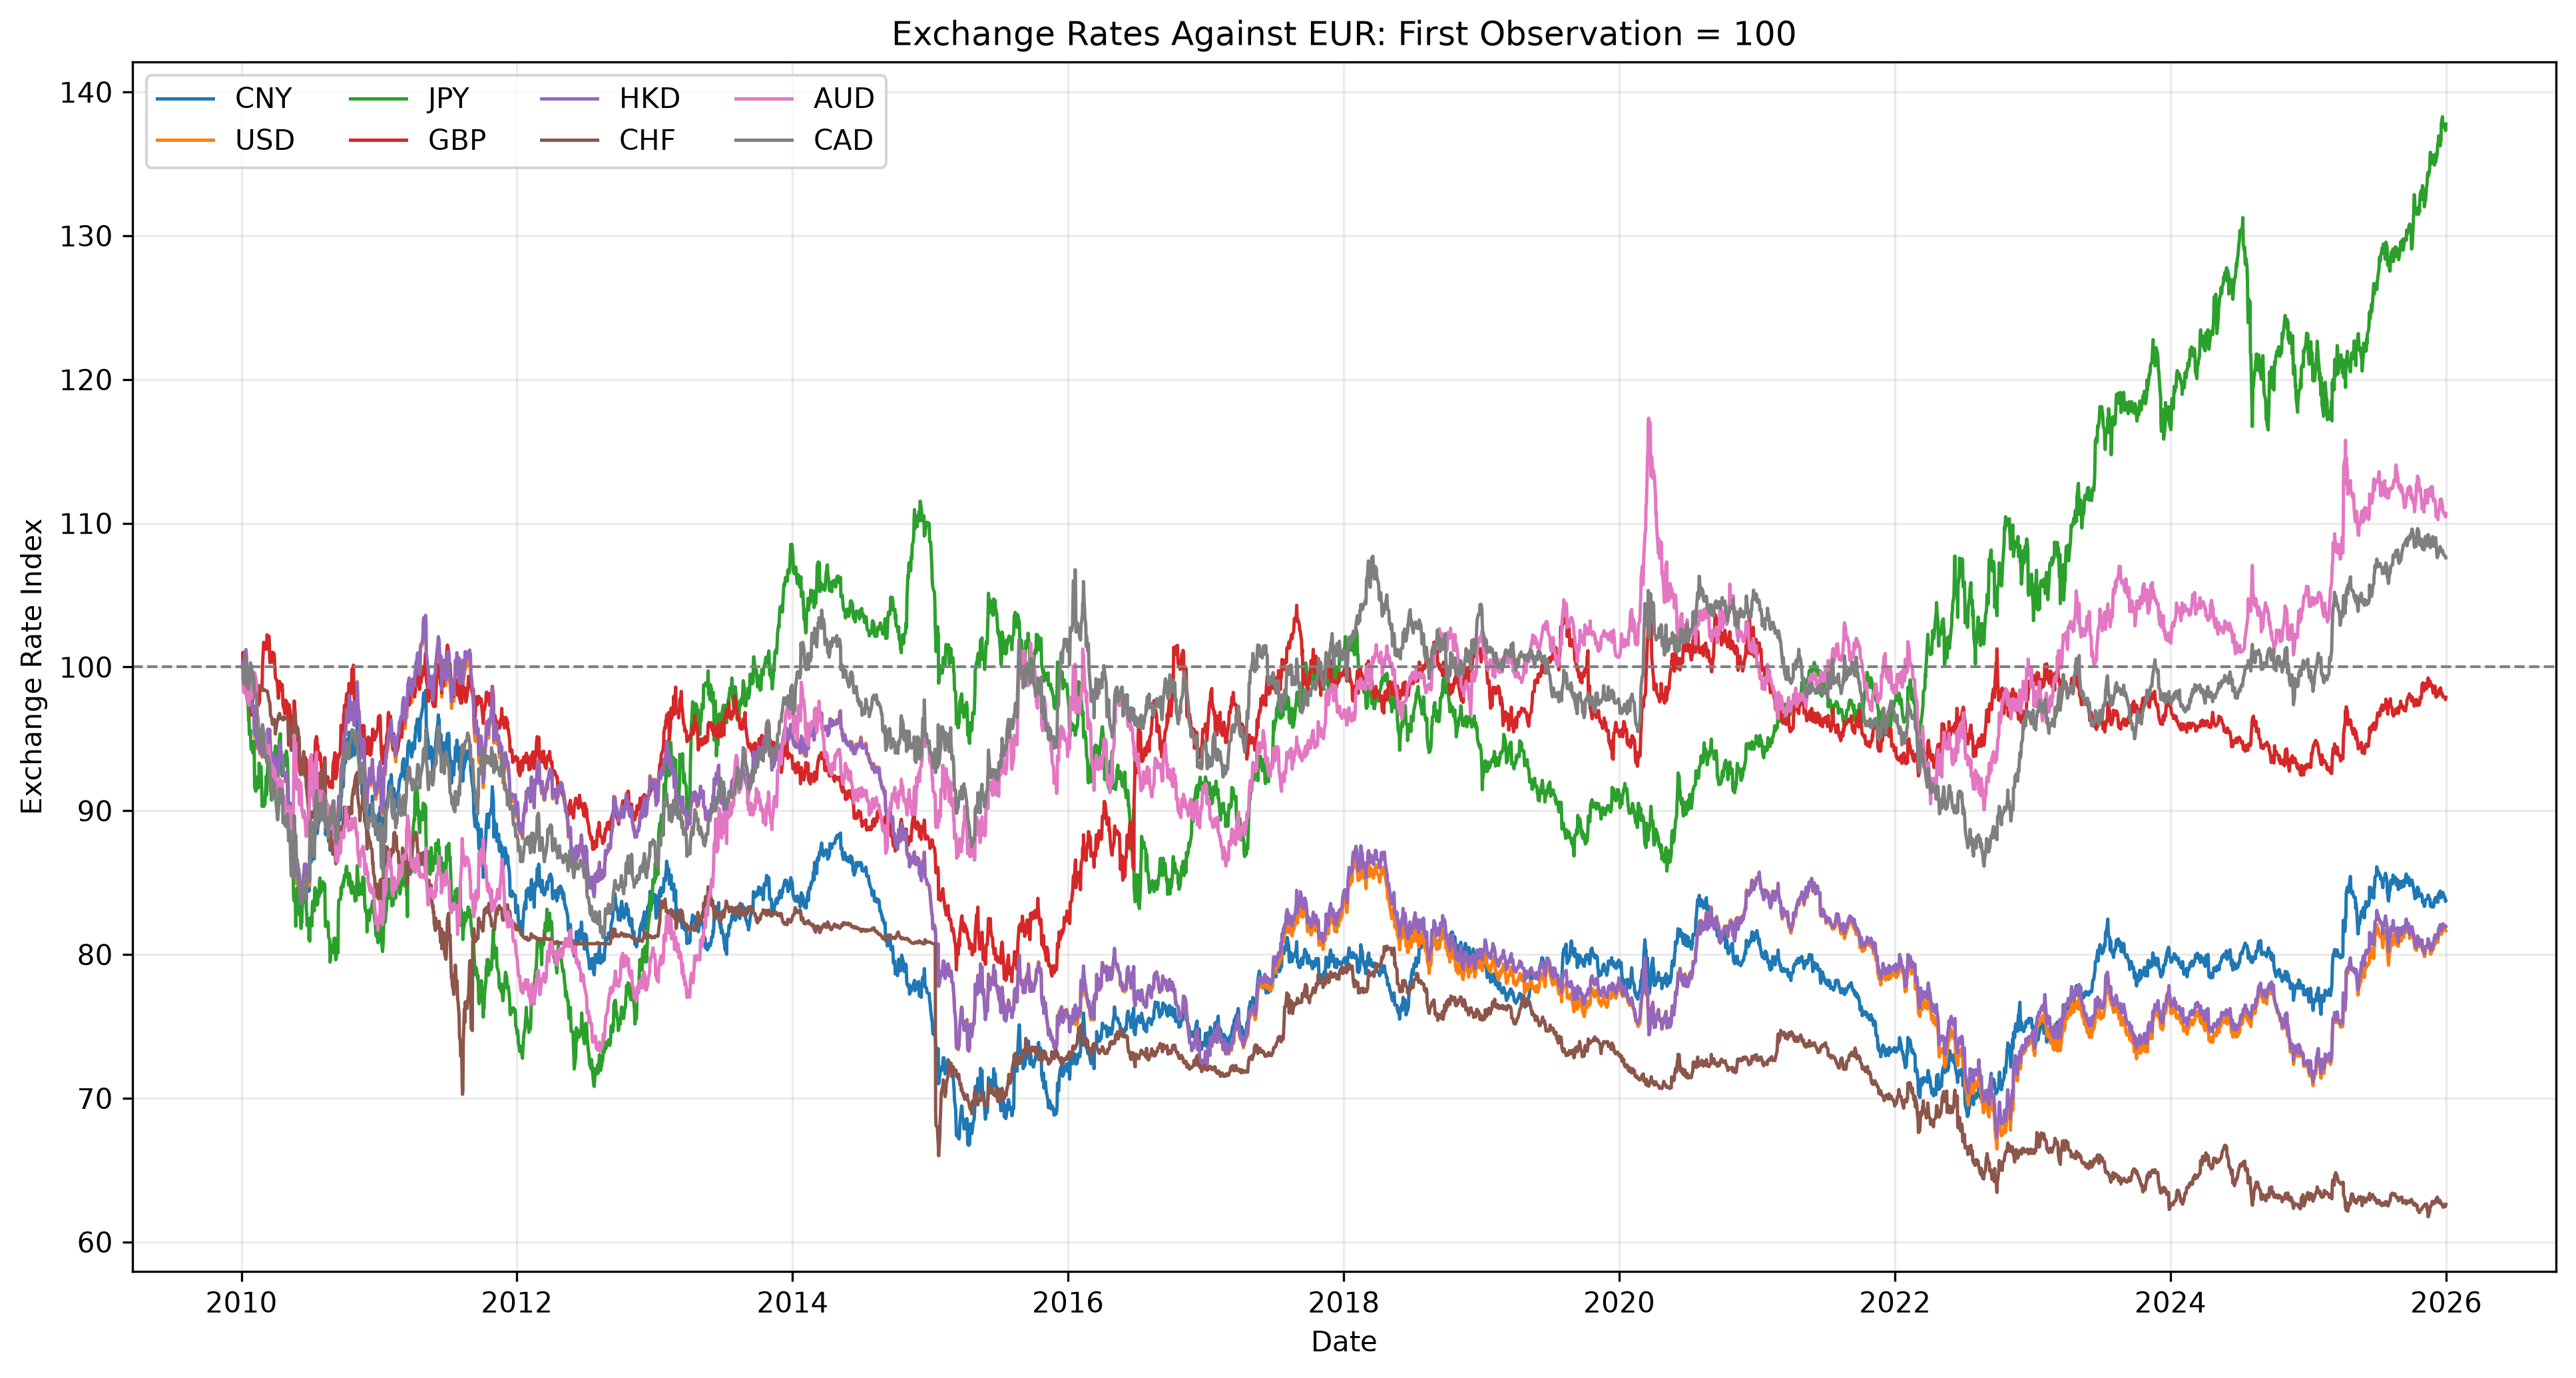
\includegraphics[width=0.95\textwidth]{figures/fig_trends.png}
\caption{Indexed exchange rates against the euro, first observation = 100. The series are plotted on a common scale; the dashed line marks the base value.}
\label{fig:trends}
\end{figure*}

\begin{figure*}[t]
\centering
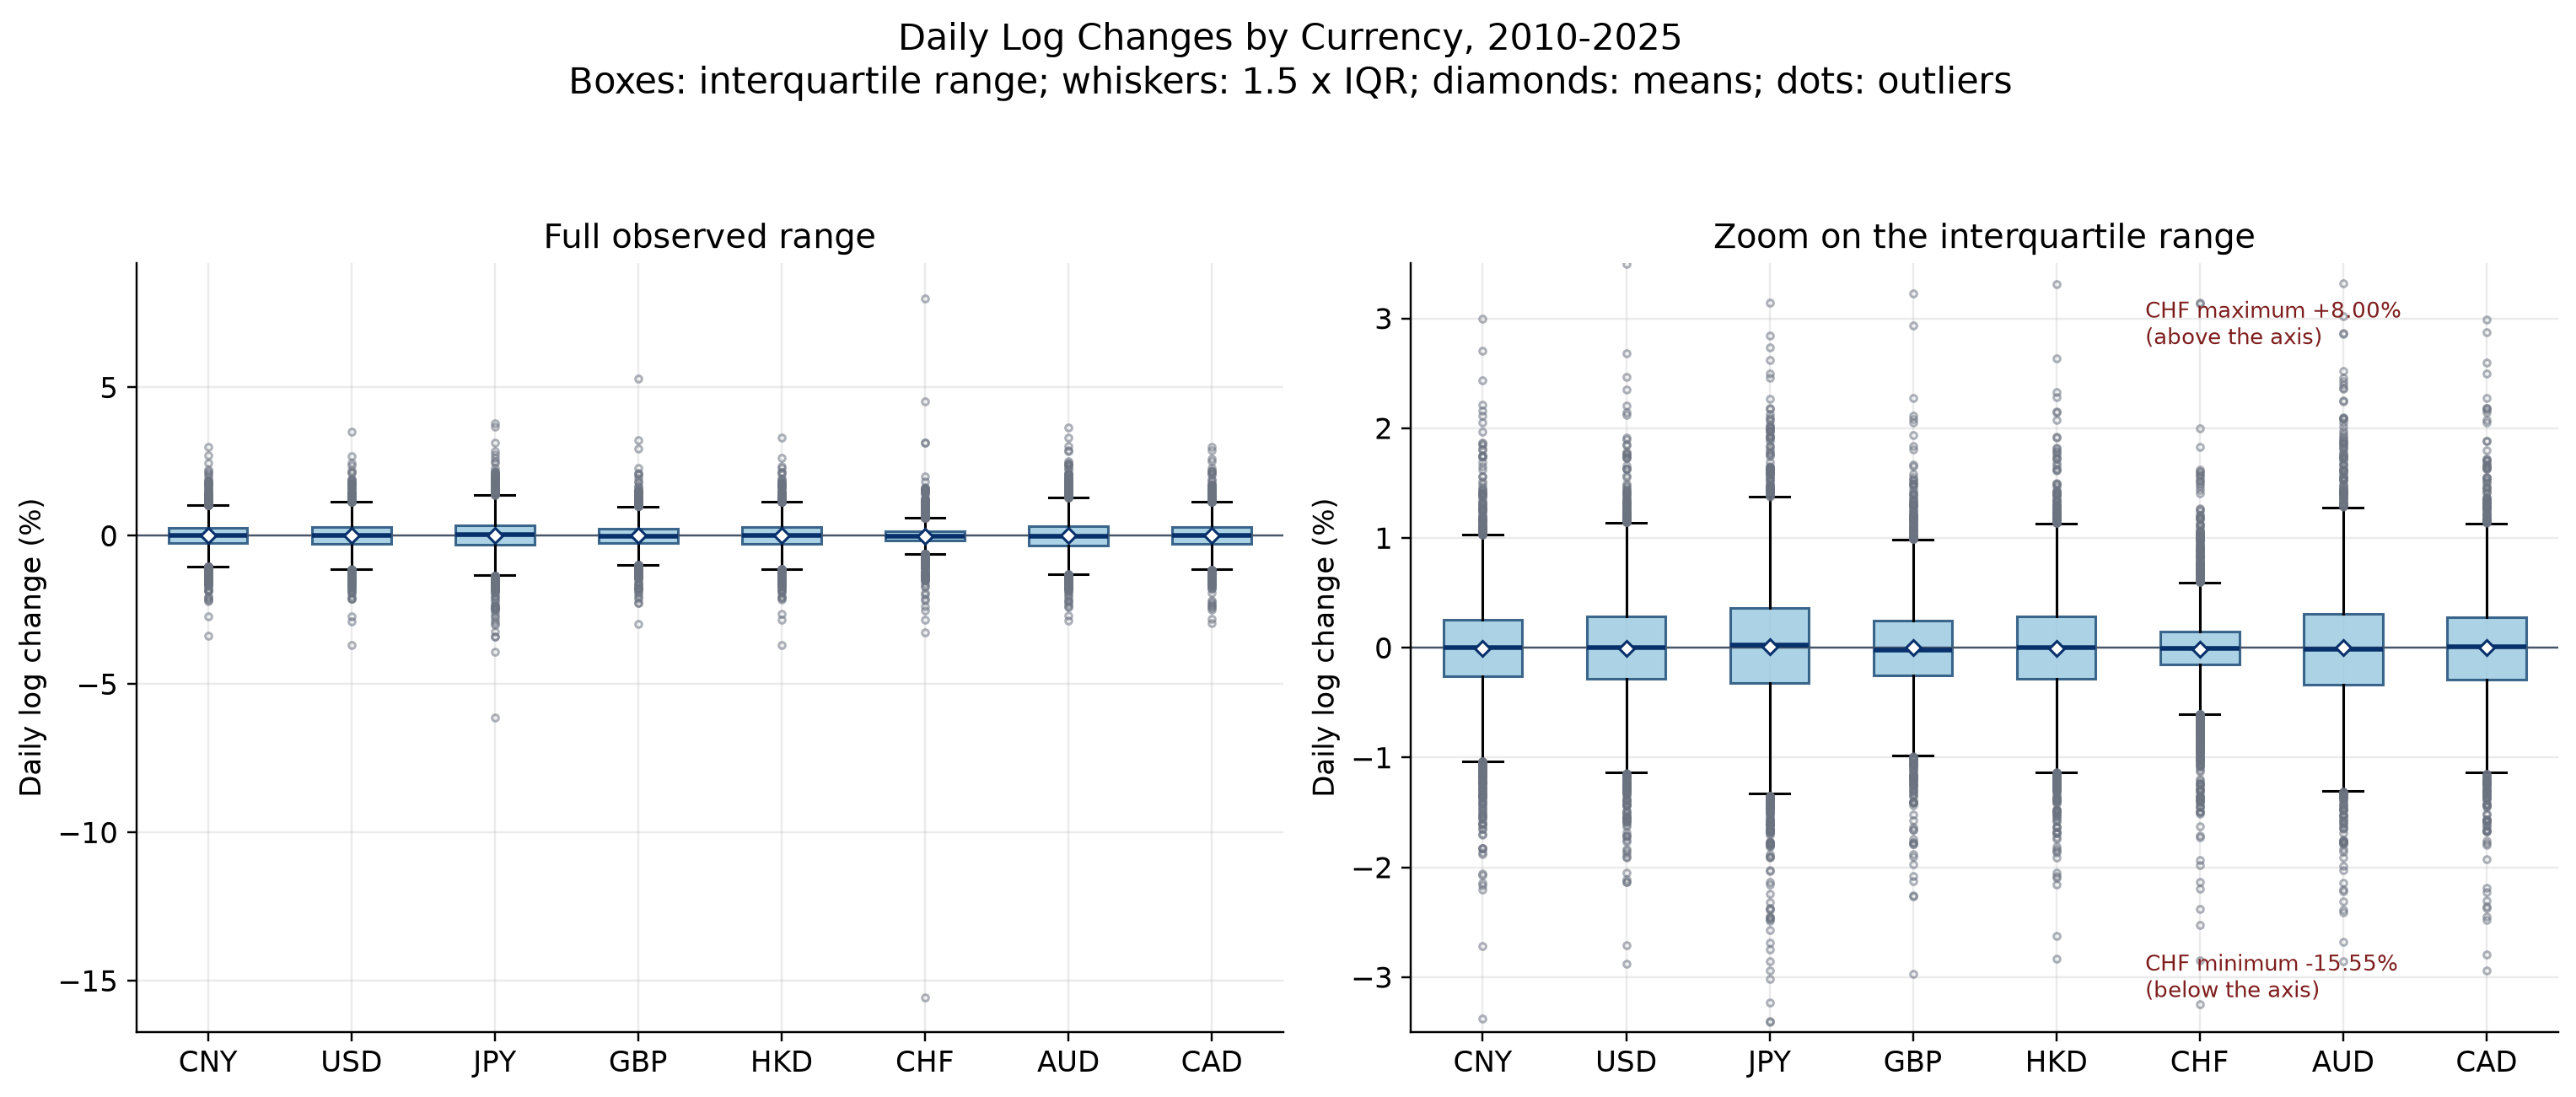
\includegraphics[width=0.95\textwidth]{figures/fig_boxplots.png}
\caption{Daily log changes by currency. The left panel shows the full observed range; the right panel zooms on the interquartile range and annotates the CHF extremes. Whiskers extend to 1.5 times the interquartile range; dots are outliers.}
\label{fig:boxplots}
\end{figure*}

Figure~\ref{fig:scatter} adds the pairwise view. Points for USD--HKD lie almost on a line, while CHF--AUD forms a cloud with a shallow slope; the coefficient alone would not show that difference.

\begin{figure*}[t]
\centering
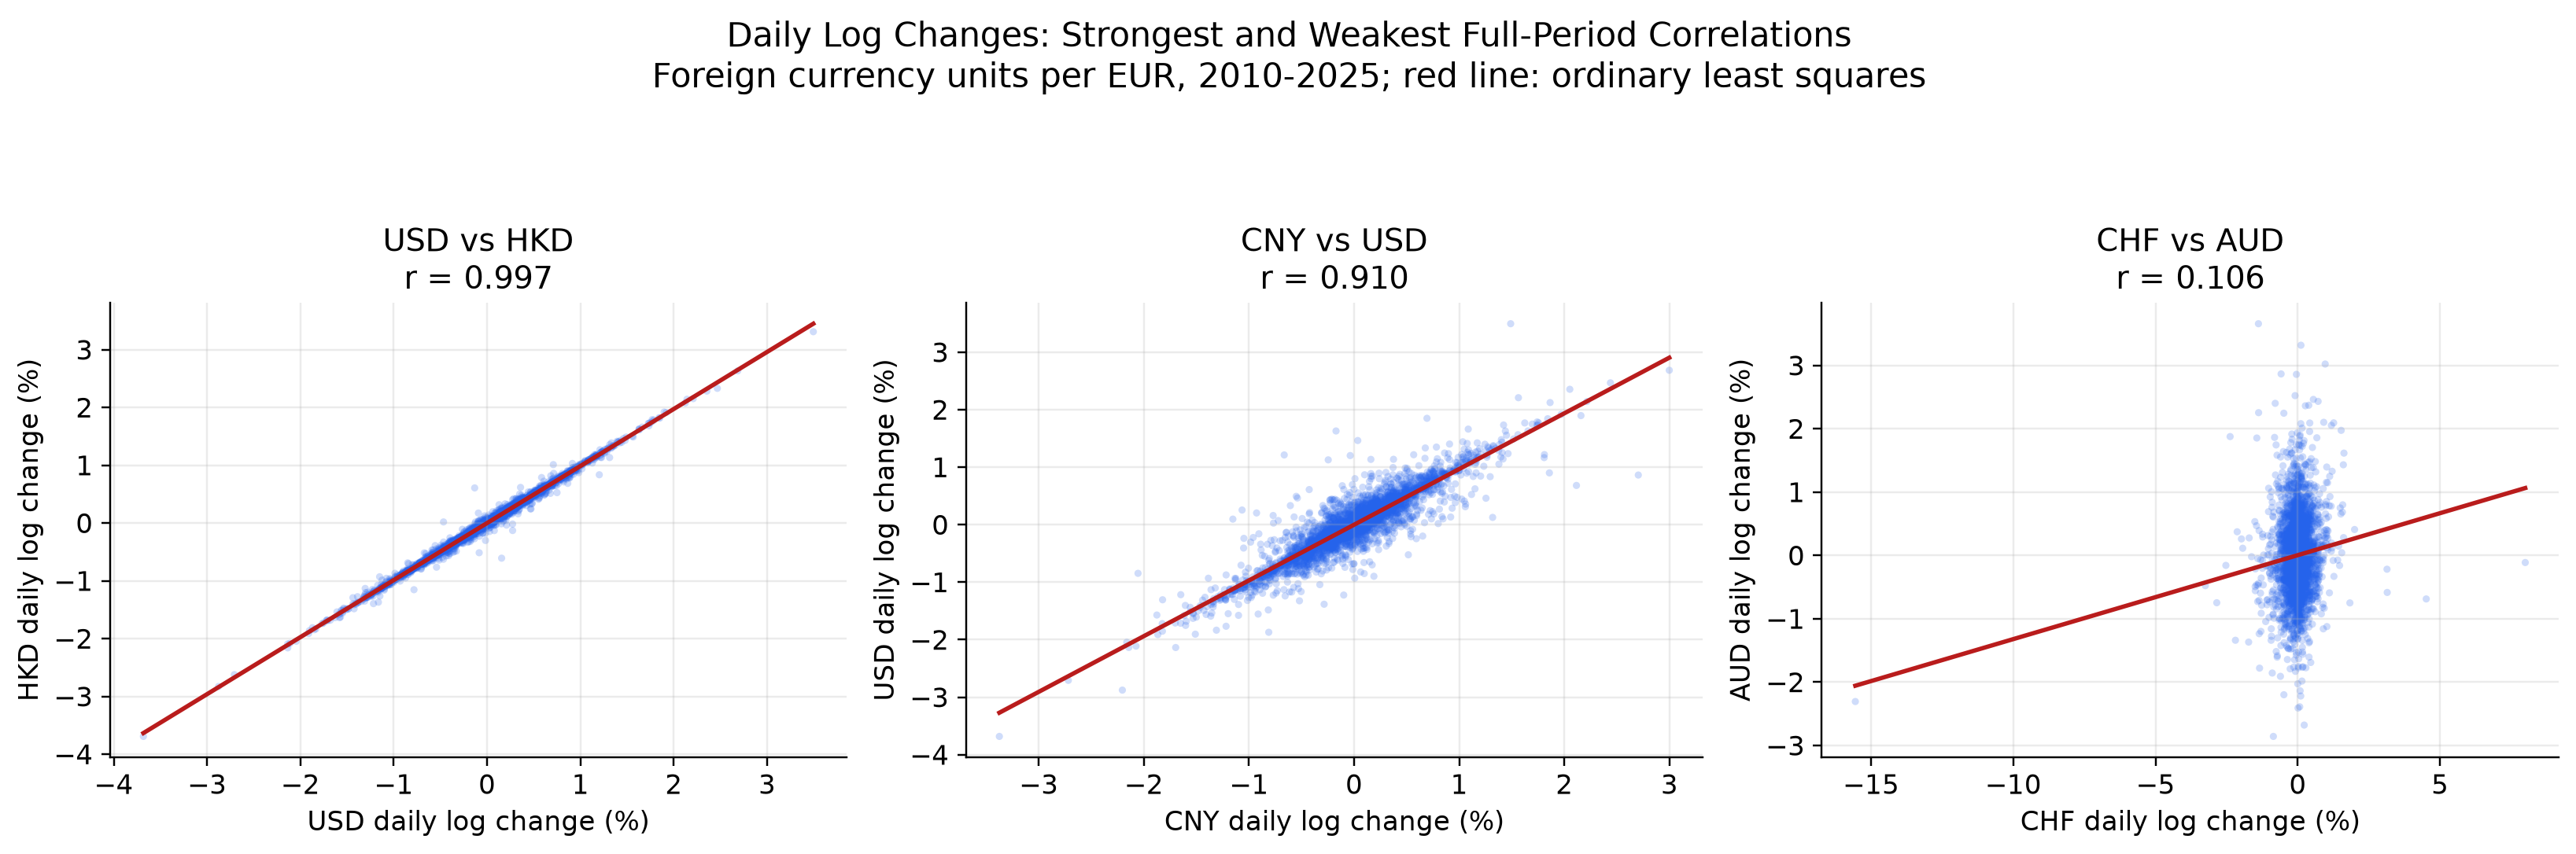
\includegraphics[width=0.92\textwidth]{figures/fig_scatter.png}
\caption{Daily log changes for USD--HKD, CNY--USD and CHF--AUD. The red line is an ordinary least squares fit. The first panel is the near-deterministic pair; the last is the weakest full-period pair.}
\label{fig:scatter}
\end{figure*}

Figure~\ref{fig:hist} adds the full distribution panels. Bins and axes are shared, so the tails can be compared across currencies; the log count axis keeps the large central mass and the sparse tails on one scale.

\begin{figure}[t]
\centering
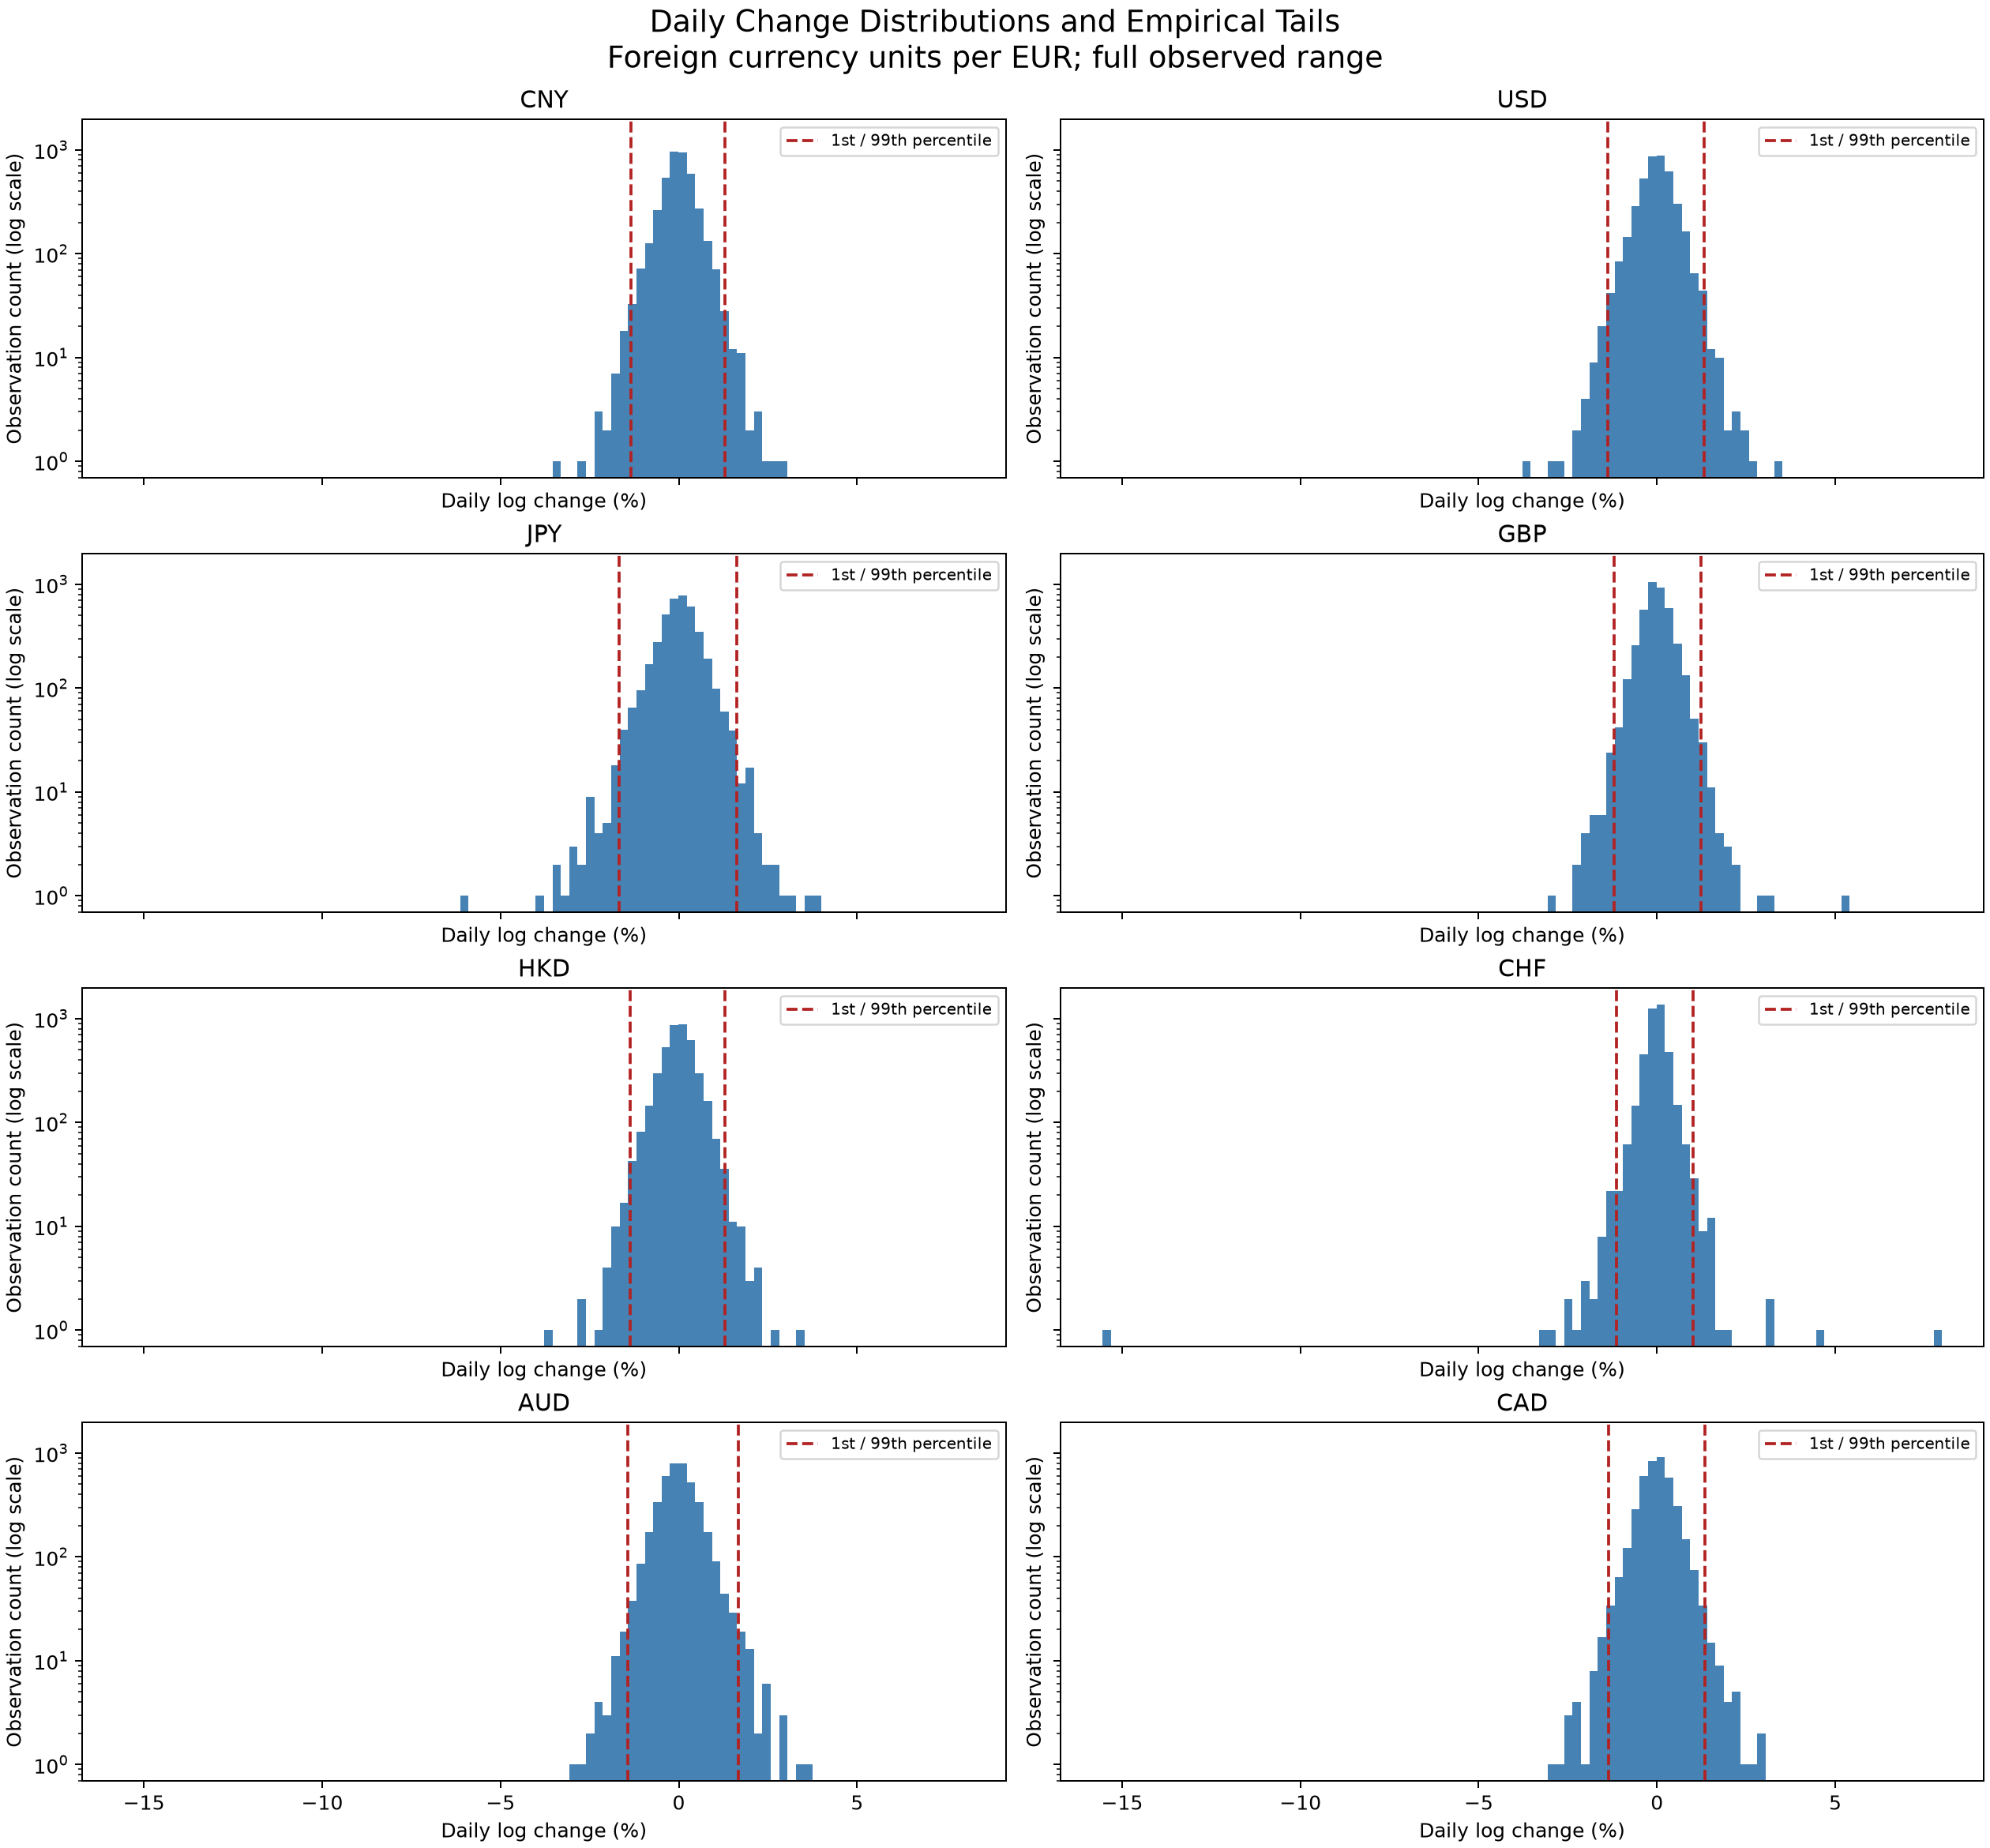
\includegraphics[width=\columnwidth]{figures/fig_hist.png}
\caption{Empirical distributions of daily log changes by currency. Bins and axes are shared; the dashed lines mark the 1st and 99th percentiles. The vertical axis is on a log scale.}
\label{fig:hist}
\end{figure}

\subsection{Challenges}
Four properties of the data shape the rest of the analysis. First, all quotes share the euro as the base. A common euro movement pushes many quotes in the same direction, so positive correlation is partly a base effect rather than evidence of bilateral dependence. We return to this point when interpreting the correlation matrix.

Second, rolling windows overlap. A 60-observation window that ends on day $t$ shares 59 observations with the window that ends on day $t+1$. The 4,037 window values are therefore not independent, and a naive standard error would be far too small. The bootstrap in Section~\ref{sec:bootstrap} uses blocks rather than individual observations for this reason, but even a block bootstrap is an approximation.

Third, the tails are heavy. CHF's 2015 move is visible in any summary that includes it, and the lower 1\% tail mean for JPY is $-2.392\%$, compared with $-1.929\%$ for CHF. A single statistic can be dominated by a handful of sessions. We report both the full-sample and outlier-excluded versions rather than choosing one silently.

Fourth, these are reference rates, not transaction prices. Successive observations can span weekends and holidays, so daily changes are not uniformly spaced 24-hour returns. The data are also a small cross-section: eight currencies and one 16-year sample. The conclusions describe this sample, and the report avoids claims about future probabilities or causal mechanisms.

\subsection{System Design}
\label{sec:system}
The implementation is a set of scripts rather than one application. Each stage reads a fixed input, writes a fixed output, and resolves paths relative to its own location; Table~\ref{tab:system} summarises the chain. The analysis and benchmark stages are deliberately separate: the benchmark imports the same pair function as the baseline, but correctness validation and CSV I/O sit outside the timed region. The figure stage reads the saved CSV summaries, so figures can be rebuilt without re-running the experiments.

\begin{table}[t]
\caption{System design: data-flow stages and outputs.}
\label{tab:system}
\centering
\small
\renewcommand{\arraystretch}{1.15}
\begin{tabularx}{\columnwidth}{@{}l>{\raggedright\arraybackslash}X>{\raggedright\arraybackslash}X@{}}
\toprule
Stage & Function & Output \\
\midrule
Acquisition & ECB snapshot, period and currency filter & cleaned rates \\
Transform & daily log changes; month-end changes & return tables \\
Analysis & correlation, clustering, volatility & matrices, clusters, volatility \\
Robustness & window, outlier, bootstrap & sensitivity tables \\
Benchmark & serial, pool, scaling, chunksize & timing tables, figures \\
Reproduction & rebuild all figures from saved CSVs & 22 figures \\
\bottomrule
\end{tabularx}
\end{table}

% --------------------------------------------------------------------------
\section{Validation Strategy}
\label{sec:validation}

\subsection{Numerical checks}
There is no train/test split in this project because there is no predictive model. Validation here means that the computations are correct, the reported numbers can be reproduced, and the conclusions survive reasonable changes in the analysis choices. The pipeline uses four kinds of checks.

The first is structural. Dates must be unique and sorted, the eight series must be finite, and exchange-rate levels must be positive. The cleaning script stops on a failed check rather than dropping the offending rows.

The second is arithmetic. The first 60-observation rolling volatility is compared with a direct sample standard deviation of the first 60 changes. The rolling-correlation outputs are checked for missing values, and the parallel versions are compared element by element with the serial reference. Monthly changes are compounded and compared with the ratio of the final and initial month-end quotes. These checks catch window-alignment errors, which are easy to introduce when a rolling result is shifted or sliced.

The third is parallel correctness. Every parallel result is compared with the serial reference using \texttt{allclose} at \texttt{rtol}$=10^{-10}$ and \texttt{atol}$=10^{-12}$. The comparison runs outside the timed region, so the measurement does not include validation overhead. In the 28-pair benchmark the maximum absolute difference is zero; in the scaling experiment the same tolerance is applied to a checksum and four summary statistics per pair.

The fourth is cross-file consistency. The bootstrap checks its baseline correlations against the saved full-period table (within the six-decimal storage rounding), and the sensitivity scripts require the two event dates to exist in the sample. The figure-regeneration script rebuilds all 22 figures from code and fails if any expected file is missing.

\subsection{Leakage and multiple comparisons}
The rolling correlation at date $t$ uses observations $t-59$ through $t$; no future observation enters the window. The full-period correlation and the clustering use the whole sample, but they are descriptive summaries, not predictions, so a train/test split has no meaning here. The relevant leakage risk is in the parallel implementation: a worker must receive the same data and the same window definition as the serial reference. The element-wise comparison in Section~\ref{sec:parallel} is the check for that.

With 28 pairs, some correlations will look interesting by chance. We do not report p-values or a family-wise error rate, because the analysis is not framed as a null-hypothesis test. Instead we report bootstrap intervals and a rank-stability check after removing the two extreme dates. This is a weaker claim, and the report says so where it matters. A reader who needs formal inference should treat the intervals as descriptive, not confirmatory.

% --------------------------------------------------------------------------
\section{Baseline Analysis}
\label{sec:baseline}

\subsection{Full-period structure}
The baseline is the full-period descriptive analysis: the correlation matrix, the hierarchical clustering and the serial rolling-correlation implementation. All 28 full-period correlations are positive. The strongest pair is USD--HKD ($r = 0.9966$), followed by CNY--HKD (0.9110) and CNY--USD (0.9098). The weakest are CHF--AUD (0.1064), JPY--AUD (0.1464) and GBP--CHF (0.1466). The USD--HKD result is not surprising: the Hong Kong dollar is linked to the US dollar, and both quotes are expressed against the euro. The weak CHF--AUD pair is more interesting because it is a full-period average of a relationship that changes sign in shorter windows.

Figure~\ref{fig:structure}(a) shows the full matrix. The visual impression matches the numbers: a dark USD--HKD cell, a moderately correlated CNY block, and a lighter CHF row. The heatmap is a summary, not a test; it does not show whether the pattern is stable.

The dendrogram in Figure~\ref{fig:structure}(b) uses average linkage and the distance $\sqrt{2(1-r)}$. USD and HKD merge first at 0.0829, CNY joins at 0.4233, AUD and CAD merge at 0.8793, JPY joins the CNY--USD--HKD group at 0.9964, and GBP joins the AUD--CAD pair at 1.0964. CHF is the last currency to join, at 1.2410. Cutting the tree into two, three and four clusters gives the expected nested partitions; the four-cluster cut separates AUD and CAD from GBP, while CHF remains a singleton. We treat the partitions as exploratory. No optimal number of clusters is claimed, and the result depends on the period, the common base, the distance and the linkage rule.

\begin{figure*}[t]
\centering
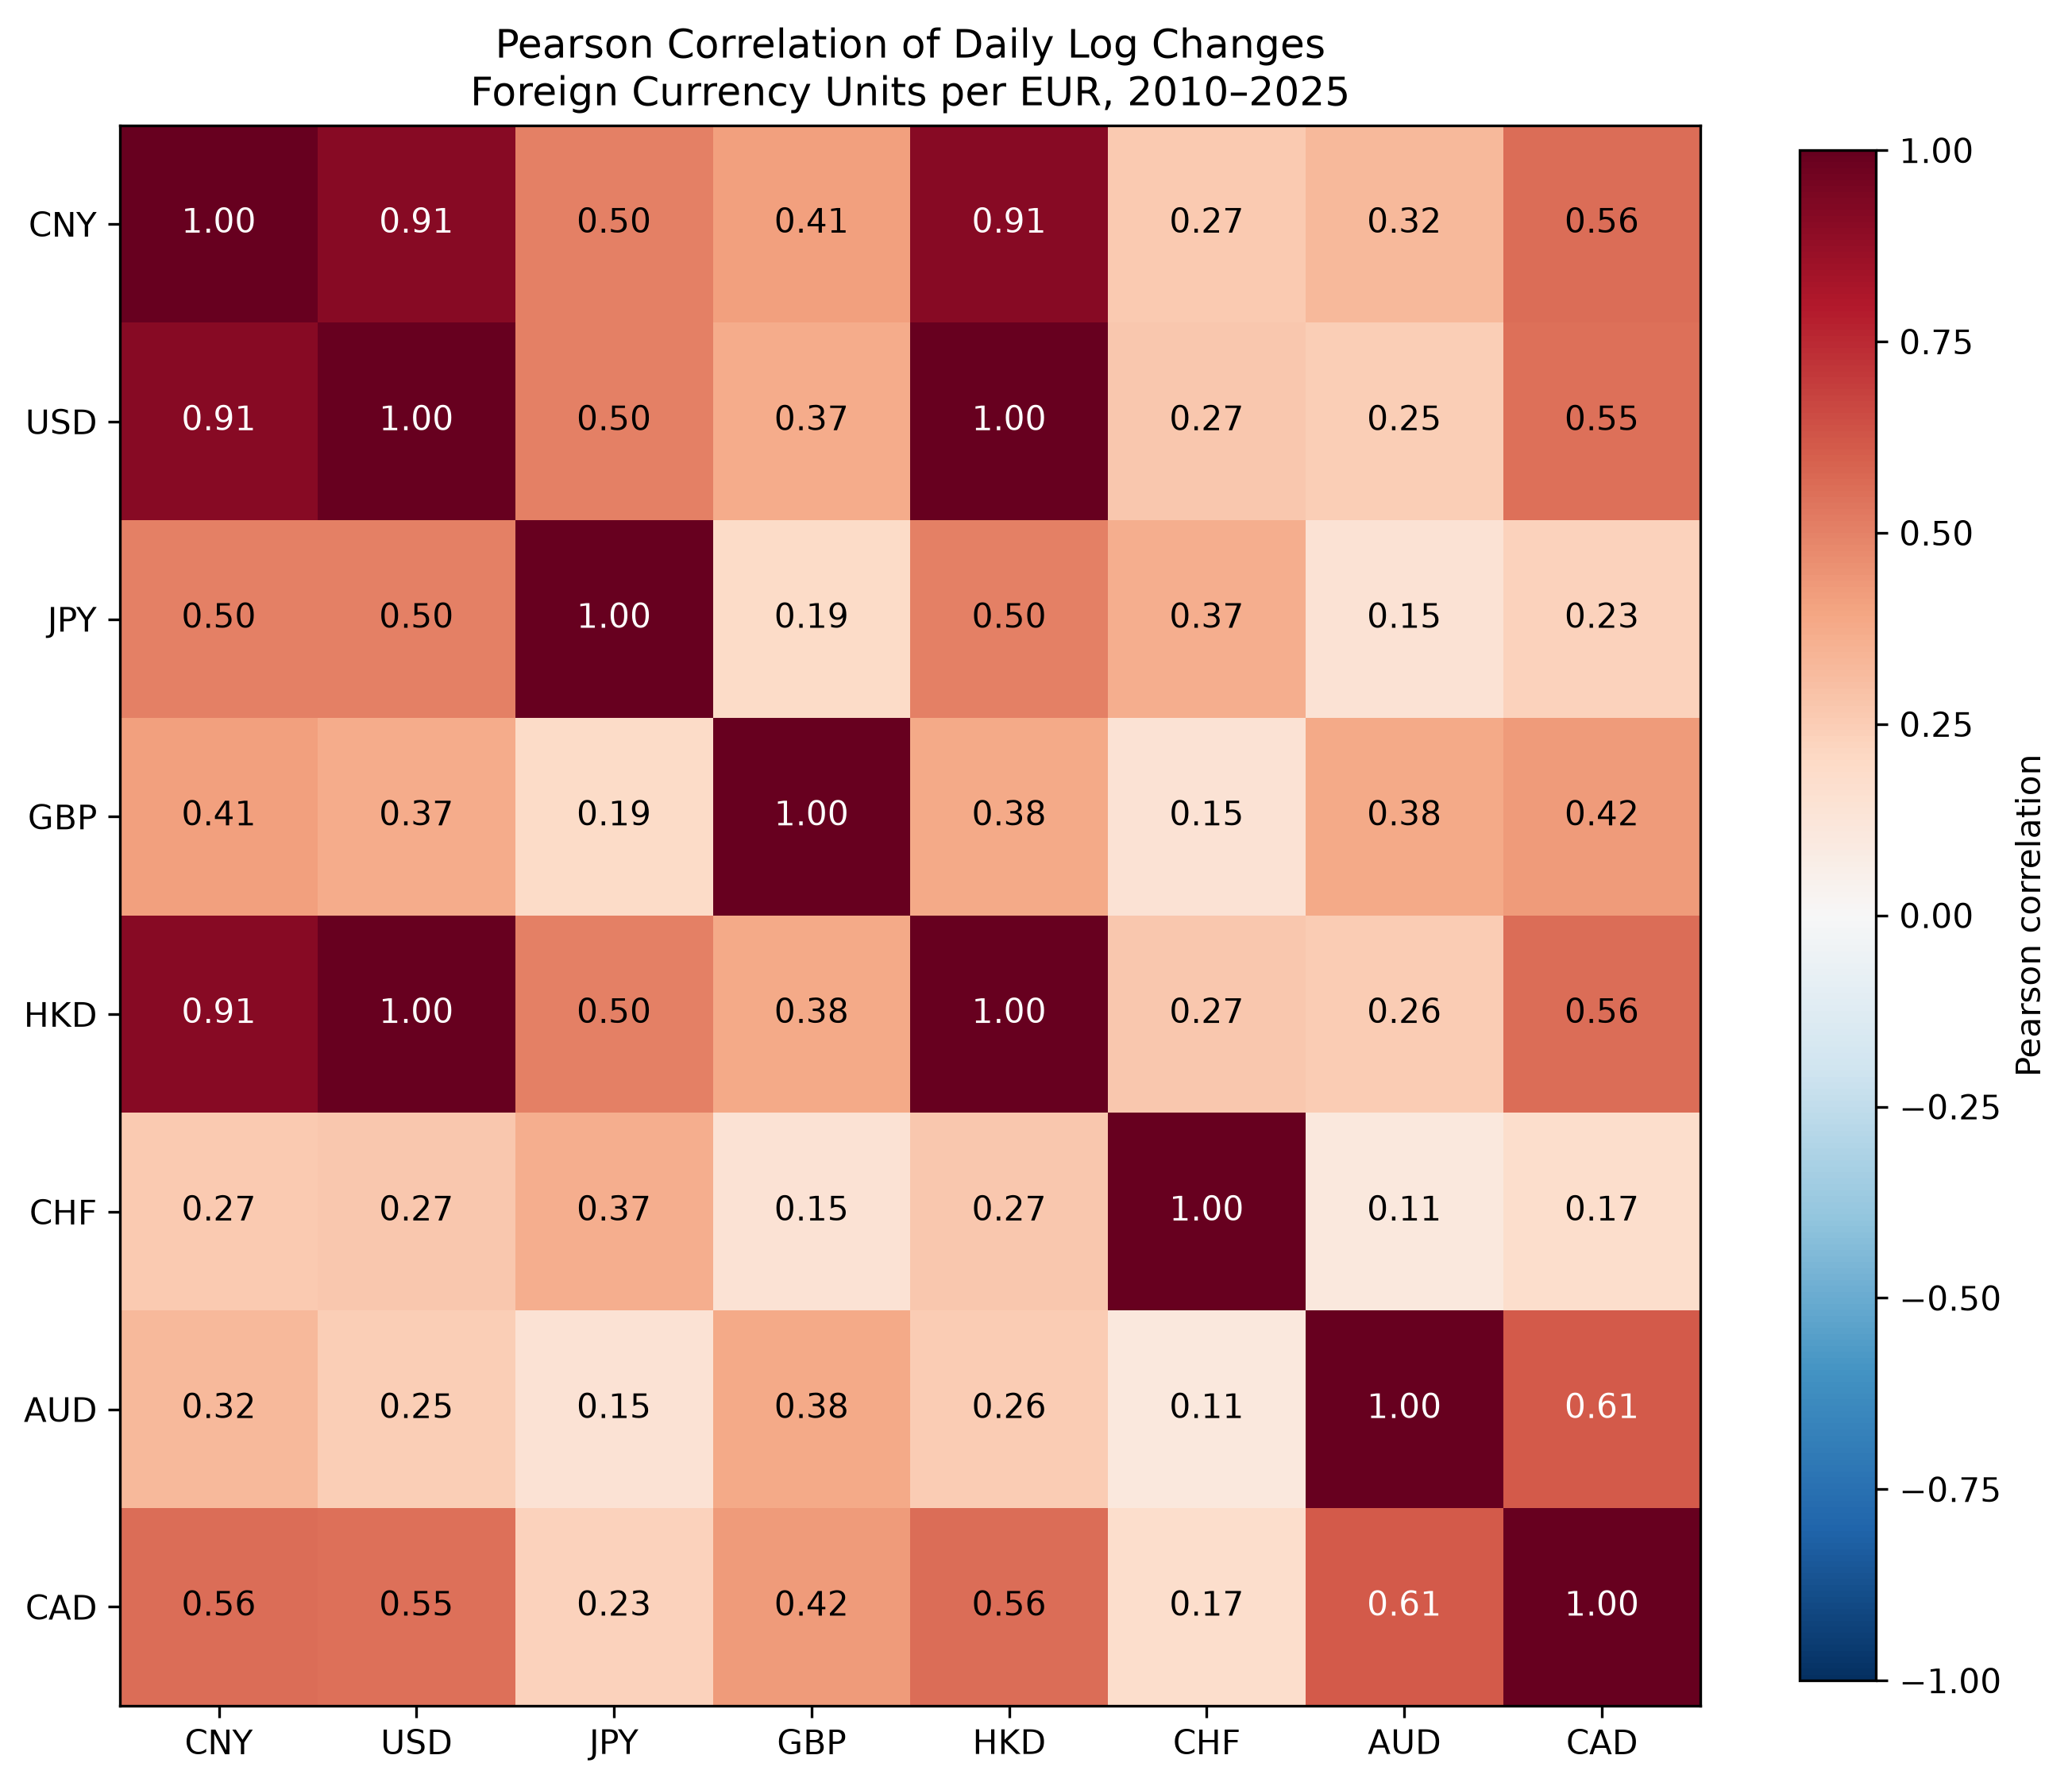
\includegraphics[width=0.46\textwidth]{figures/fig_heatmap.png}\hfil
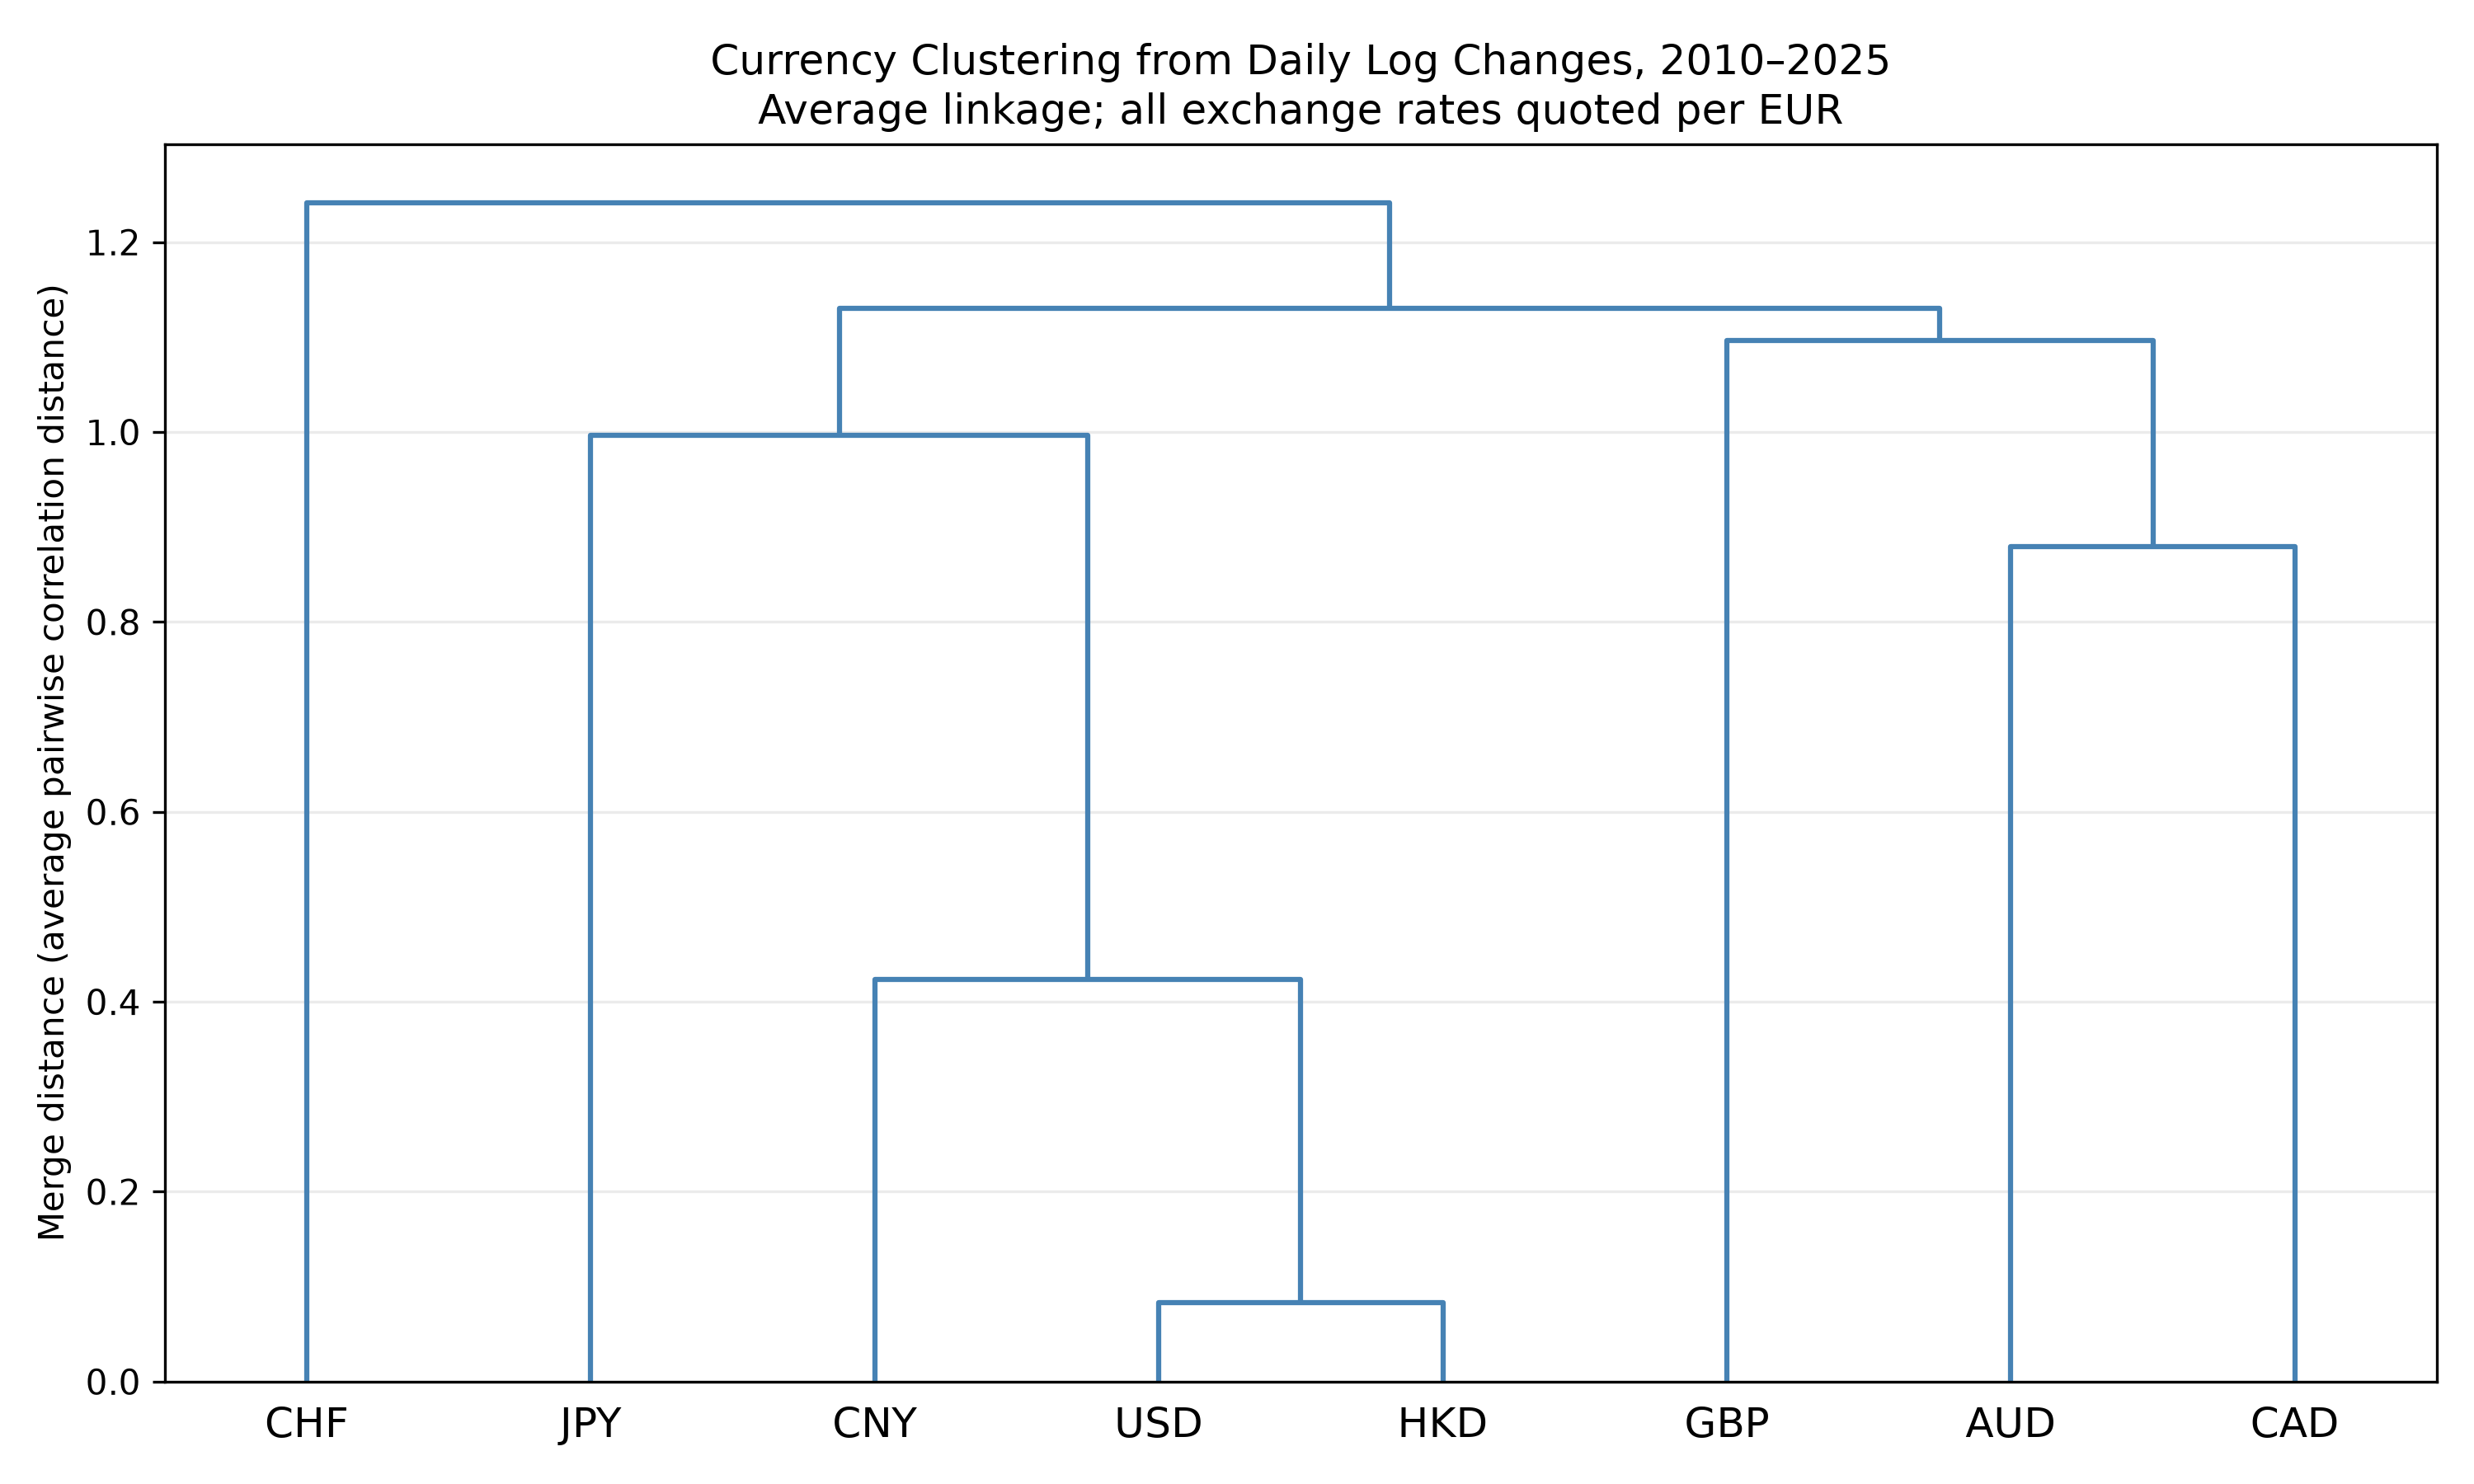
\includegraphics[width=0.46\textwidth]{figures/fig_dendrogram.png}
\caption{Full-period correlation structure. (a) Pearson correlations of daily log changes. (b) Average-linkage dendrogram using the distance $\sqrt{2(1-r)}$; the vertical axis is the merge distance.}
\label{fig:structure}
\end{figure*}

\subsection{Rolling baseline and serial cost}
A 60-observation window produces 4,037 valid windows per pair. The rolling correlations are not a small perturbation of the full-period values. USD--HKD stays between 0.9163 and 0.99999, with a standard deviation of 0.0092. JPY--AUD moves from $-0.6009$ to 0.8077, with a standard deviation of 0.2597. USD--JPY has the largest rolling standard deviation (0.2723), even though its full-period correlation is a moderate 0.5050. Figure~\ref{fig:rolling} shows four pairs: the near-flat USD--HKD line, the slowly declining CNY--USD line, the AUD--CAD line, and the sign-changing AUD--JPY line.

\begin{figure*}[t]
\centering
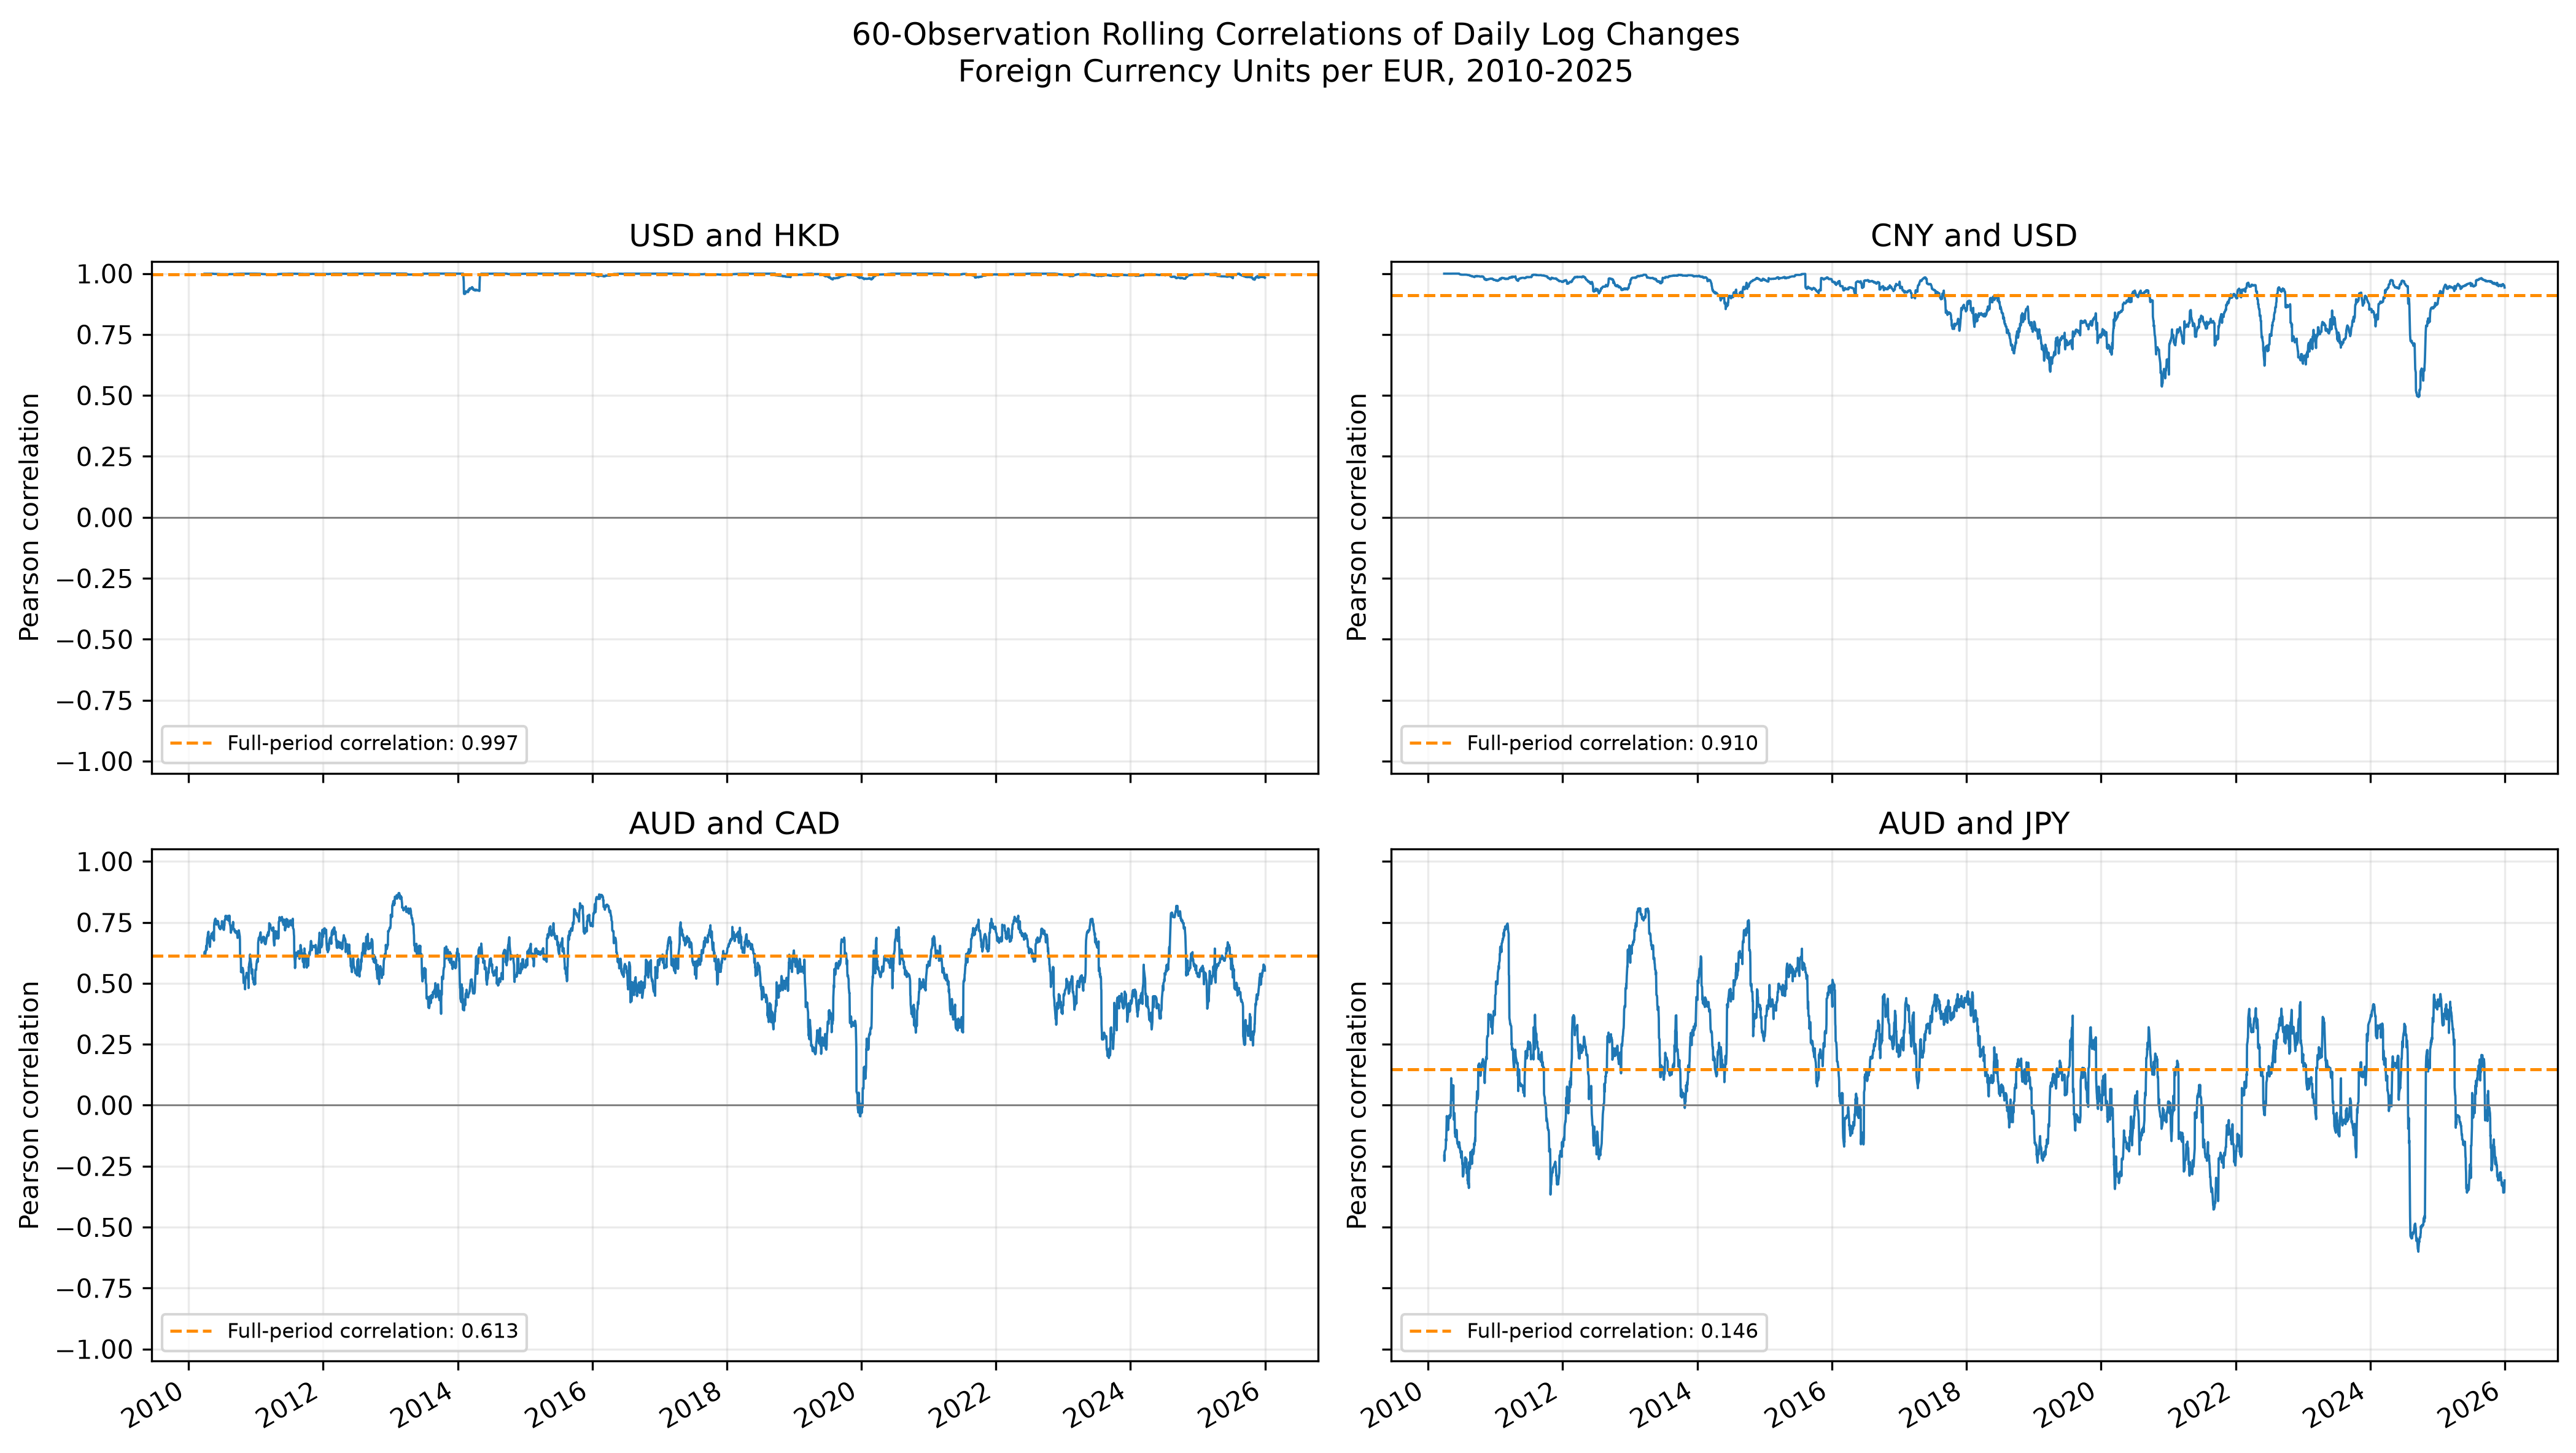
\includegraphics[width=0.95\textwidth]{figures/fig_rolling.png}
\caption{60-observation rolling Pearson correlations for four representative pairs. The dashed line is the full-period correlation; the horizontal line marks zero.}
\label{fig:rolling}
\end{figure*}

The serial implementation computes all 28 pairs in one process. On the test machine (Python 3.11.9, pandas 3.1.1, 16 logical CPUs) the median serial time is 17.9--18.6 ms over ten repetitions. That number is the baseline for the parallel experiments. It is small enough that process start-up and message passing are plausible bottlenecks, which is exactly why the workload is useful for a parallel study.

% --------------------------------------------------------------------------
\section{Improvements}
\label{sec:improvements}

\subsection{Window and outlier sensitivity}
\label{sec:sensitivity}
The 60-observation window is a reporting choice, not an estimated optimum. We recompute four pairs with 30, 60 and 120 observations. The ordering of pair variability is stable across windows: USD--HKD is the least variable, AUD--JPY the most variable, and CNY--USD and AUD--CAD fall in between. The magnitudes change. USD--HKD's rolling standard deviation is 0.0124 at 30 observations, 0.0092 at 60 and 0.0068 at 120. AUD--JPY's values are 0.3009, 0.2597 and 0.2228. Longer windows smooth the series; shorter windows are noisier. A report that showed only the 60-observation figure would understate how much the choice matters for the level of variability, even though it does not change the ranking.

The two extreme sessions are handled separately. Dropping 2015-01-15 \cite{snb2015} and 2016-06-24 \cite{ec2016} changes the correlation vector only modestly: the Spearman rank correlation between the baseline and the outlier-excluded vector is 0.9956. The largest absolute change is JPY--CHF, from 0.3663 to 0.4203 ($+0.0541$). The next largest changes all involve CHF: USD--CHF ($+0.0354$), HKD--CHF ($+0.0347$) and CNY--CHF ($+0.0332$). The CHF daily volatility falls from 0.4632\% to 0.3944\% ($-0.0688$ percentage points); GBP and JPY fall by about 0.0076 and 0.0071 points, and the other currencies by less than 0.002. The ranking is robust, but the CHF level statistics are not. Both statements belong in the conclusion.

\subsection{Bootstrap intervals}
\label{sec:bootstrap}
A moving-block bootstrap provides an approximate interval for each correlation. We use blocks of 60 observations, 1,000 replicates and a fixed seed. The block length matches the rolling window and preserves short-range dependence; it is not an exact treatment of overlapping windows, and the intervals are descriptive.

The intervals separate the strong pairs from the weak ones. USD--HKD has the narrowest interval, [0.9948, 0.9977]. CNY--HKD [0.8791, 0.9329] and CNY--USD [0.8768, 0.9322] are clearly above the moderate group. The weak pairs are much less precise: JPY--GBP [0.0552, 0.2965], CHF--AUD [0.0410, 0.1712] and JPY--AUD [0.0751, 0.2258]. A point estimate near 0.1 should not be read as a precise weak relationship. Figure~\ref{fig:bootstrap} shows all 28 intervals.

\begin{figure}[t]
\centering
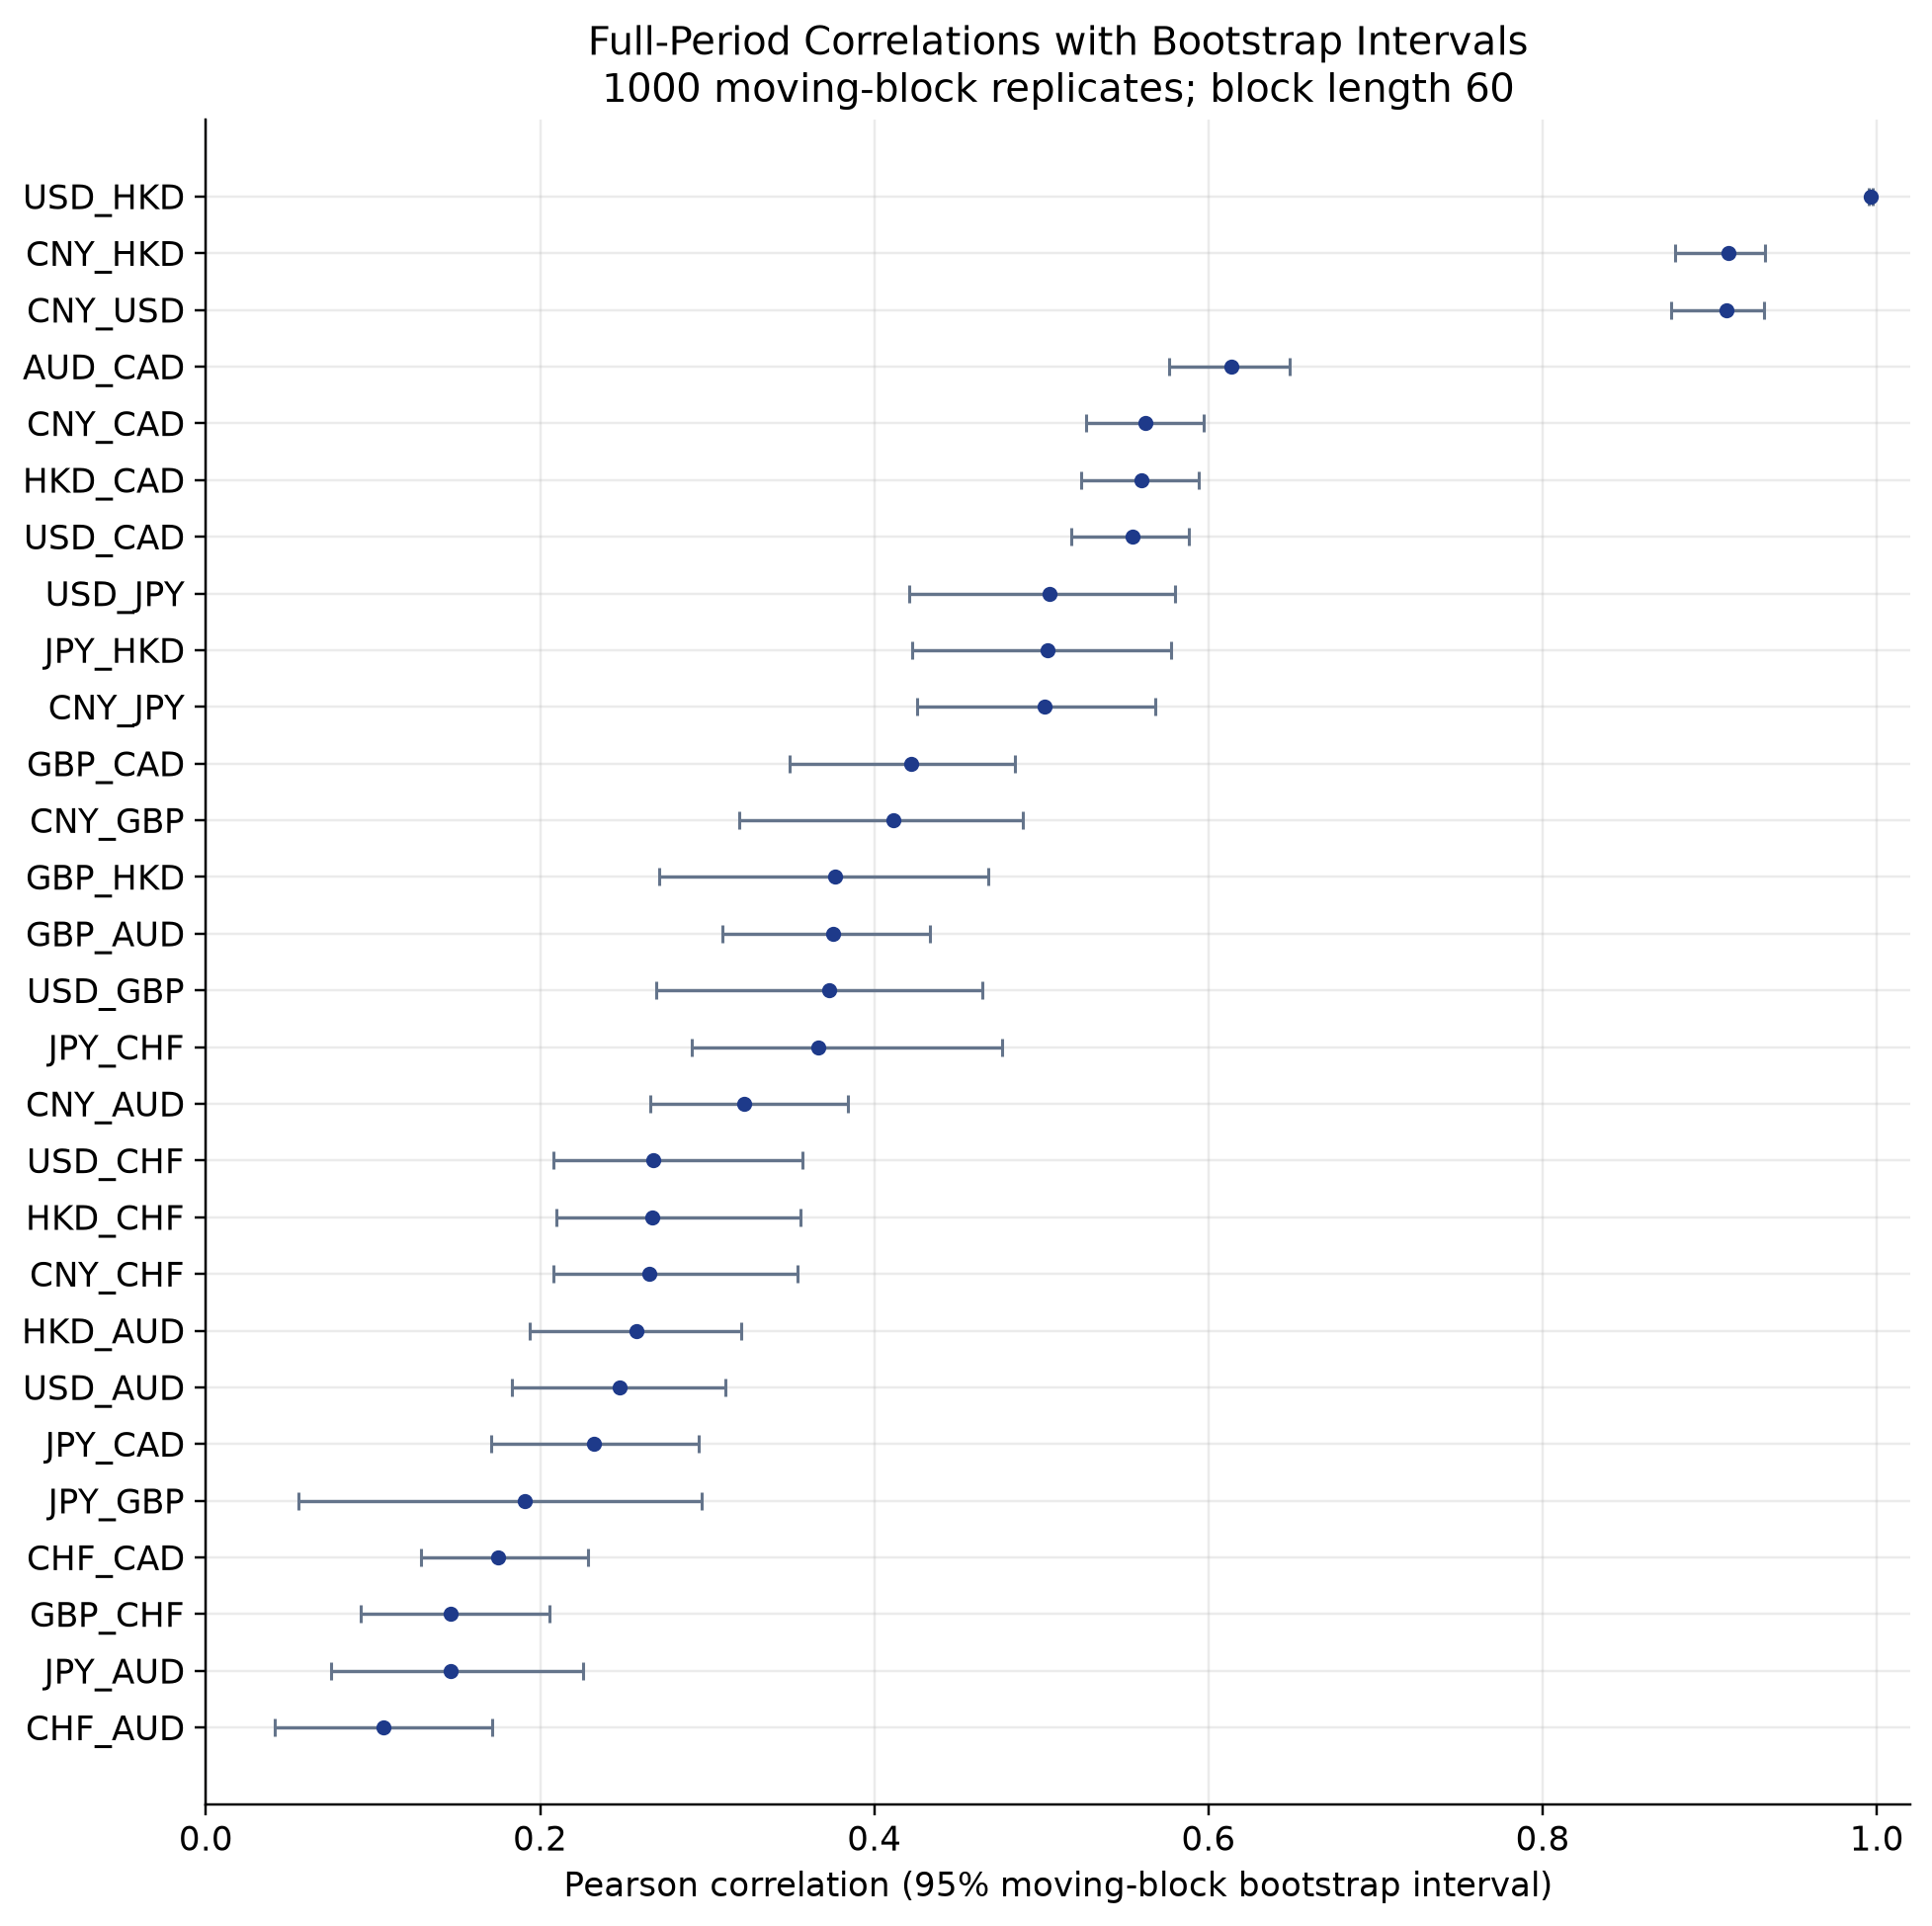
\includegraphics[width=\columnwidth]{figures/fig_bootstrap.png}
\caption{Full-period correlations with 95\% moving-block bootstrap intervals (1,000 replicates, block length 60). Pairs are ordered by their point estimate.}
\label{fig:bootstrap}
\end{figure}

\subsection{Process-pool design and the 28-pair benchmark}
\label{sec:parallel}
The workload is a list of 28 independent pair tasks. Each task computes a 60-observation rolling correlation over 4,096 changes and returns 4,037 values. We compare four configurations: serial Python, a fresh process pool \cite{python}, a reused pool, and a reused pool with batching. A barrier and a warm-up force every worker to start before timing; otherwise the lazy executor start-up leaks into the measurement. Fresh-pool timing includes process start-up, data transfer, computation, result collection and shutdown. Reused-pool timing includes transfer, computation and collection, but excludes start-up, warm-up and shutdown. Correctness validation is outside the timed region.

Table~\ref{tab:parallel} gives the medians of ten repetitions. A fresh pool is roughly 55 times slower than serial execution: 0.98--1.07 s against 17.9--18.6 ms. The reused pool without batching does not beat serial either (0.895$\times$ at two workers, 0.963$\times$ at four). Batching is what changes the result: 18.7 ms at two workers (0.960$\times$) and 11.3 ms at four workers (1.640$\times$). The best task-stage speedup is therefore 1.64$\times$, and it excludes the 0.918--1.005 s needed to create and warm the pool.

\begin{table*}[t]
\caption{28-pair rolling-correlation benchmark. Medians of ten repetitions; speedup is relative to the serial median within the same worker group. Fresh pool includes start-up and shutdown; reused pool excludes them.}
\label{tab:parallel}
\centering
\small
\renewcommand{\arraystretch}{1.15}
\begin{tabular}{lrrrr}
\toprule
 & \multicolumn{2}{c}{2 workers} & \multicolumn{2}{c}{4 workers} \\
\cmidrule(lr){2-3}\cmidrule(lr){4-5}
Method & Median (ms) & Speedup & Median (ms) & Speedup \\
\midrule
Serial & 17.915 & 1.000 & 18.551 & 1.000 \\
Fresh pool & 980.875 & 0.018 & 1,066.978 & 0.017 \\
Reused pool & 20.016 & 0.895 & 19.272 & 0.963 \\
Reused + batched & 18.667 & 0.960 & 11.313 & 1.640 \\
\bottomrule
\end{tabular}
\end{table*}

The result is easy to explain after the fact. The serial median is under 20 ms, and a process-pool message carries a fixed cost that is comparable to a large fraction of that total. Sending 28 tasks one at a time pays that cost 28 times. Batching reduces the number of messages, and four workers provide enough parallel work to recover a modest gain. The experiment does not separate start-up, serialisation, scheduling and computation; the setup measurements and the chunksize sweep in Section~\ref{sec:scaling} provide indirect evidence about which term dominates.

\subsection{Scaling, threads and chunksize}
\label{sec:scaling}
The 28-pair workload is too small to show whether the pool can scale. We therefore use synthetic factor-model series with a fixed seed and vary the number of series: 8, 16, 32 and 64, which give 28, 120, 496 and 2,016 pairs. The series have three common factors and idiosyncratic $t_5$ noise, so the pairwise correlations are a mixture of strong and weak values. The data are a benchmark device, not an empirical result. Worker-local data is broadcast once per process, and each task is a pair index; this avoids re-pickling the series for every pair and isolates computation and scheduling from data transfer. Broadcasting once also matches the memory hierarchy: the series are copied into each process's local address space once, rather than being resent for every pair, and batching keeps the queue traffic low.

Table~\ref{tab:scaling} reports the medians of five repetitions. At 2,016 pairs the serial median is 1,532.6 ms, the four-worker median is 430.1 ms (3.56$\times$) and the eight-worker median is 261.7 ms (5.86$\times$). Eight-worker efficiency is 73.2\%. At 28 pairs the eight-worker speedup is 2.76$\times$; the curve rises with workload size, which is the expected shape when a fixed overhead is amortised. An Amdahl check \cite{amdahl1967} on the medians implies a serial fraction of about 4.1\% at four workers and 5.2\% at eight. A fixed serial section would give the same value at both worker counts; the increase points to overhead that grows with the number of workers, not to a pure serial section.

\begin{table*}[t]
\caption{Scaling of the rolling-correlation workload. Medians of five repetitions; process pool with worker-local data; 60-observation windows.}
\label{tab:scaling}
\centering
\small
\renewcommand{\arraystretch}{1.15}
\begin{tabular}{rrrrrr}
\toprule
Pairs & Serial (ms) & 4 workers (ms) & 8 workers (ms) & Speedup (8w) & Efficiency (8w) \\
\midrule
28 & 21.67 & 8.32 & 7.85 & 2.76$\times$ & 0.35 \\
120 & 83.81 & 31.13 & 23.36 & 3.59$\times$ & 0.45 \\
496 & 381.09 & 123.27 & 74.17 & 5.14$\times$ & 0.64 \\
2,016 & 1,532.60 & 430.12 & 261.68 & 5.86$\times$ & 0.73 \\
\bottomrule
\end{tabular}
\end{table*}

Threads are a different story. At 2,016 pairs, a thread pool with 2, 4 and 8 threads gives 1.04$\times$, 1.09$\times$ and 1.08$\times$, respectively. The rolling correlation is not parallelised by the GIL in this implementation, and shared memory does not compensate for that. The process pool pays serialisation and start-up costs, but it is the only one of the two that scales. This is a useful negative result: it rules out the simple claim that threads are always the cheaper choice for shared-memory data.

The chunksize sweep explains the batching result. At four workers, the best chunksize is 4 (9.56 ms, 1.835$\times$); at two workers it is 7 (13.62 ms, 1.288$\times$); at eight workers it is 7 (10.08 ms, 1.739$\times$). A single chunk per workload is too coarse: at four workers, chunksize 28 takes 27.84 ms, slower than serial (0.630$\times$). The optimum is a compromise between message count and load balance, and it depends on the pair count and the worker count. Figure~\ref{fig:scaling} shows the speedup curve; Figure~\ref{fig:threads} compares the process and thread pools.

\begin{figure*}[t]
\centering
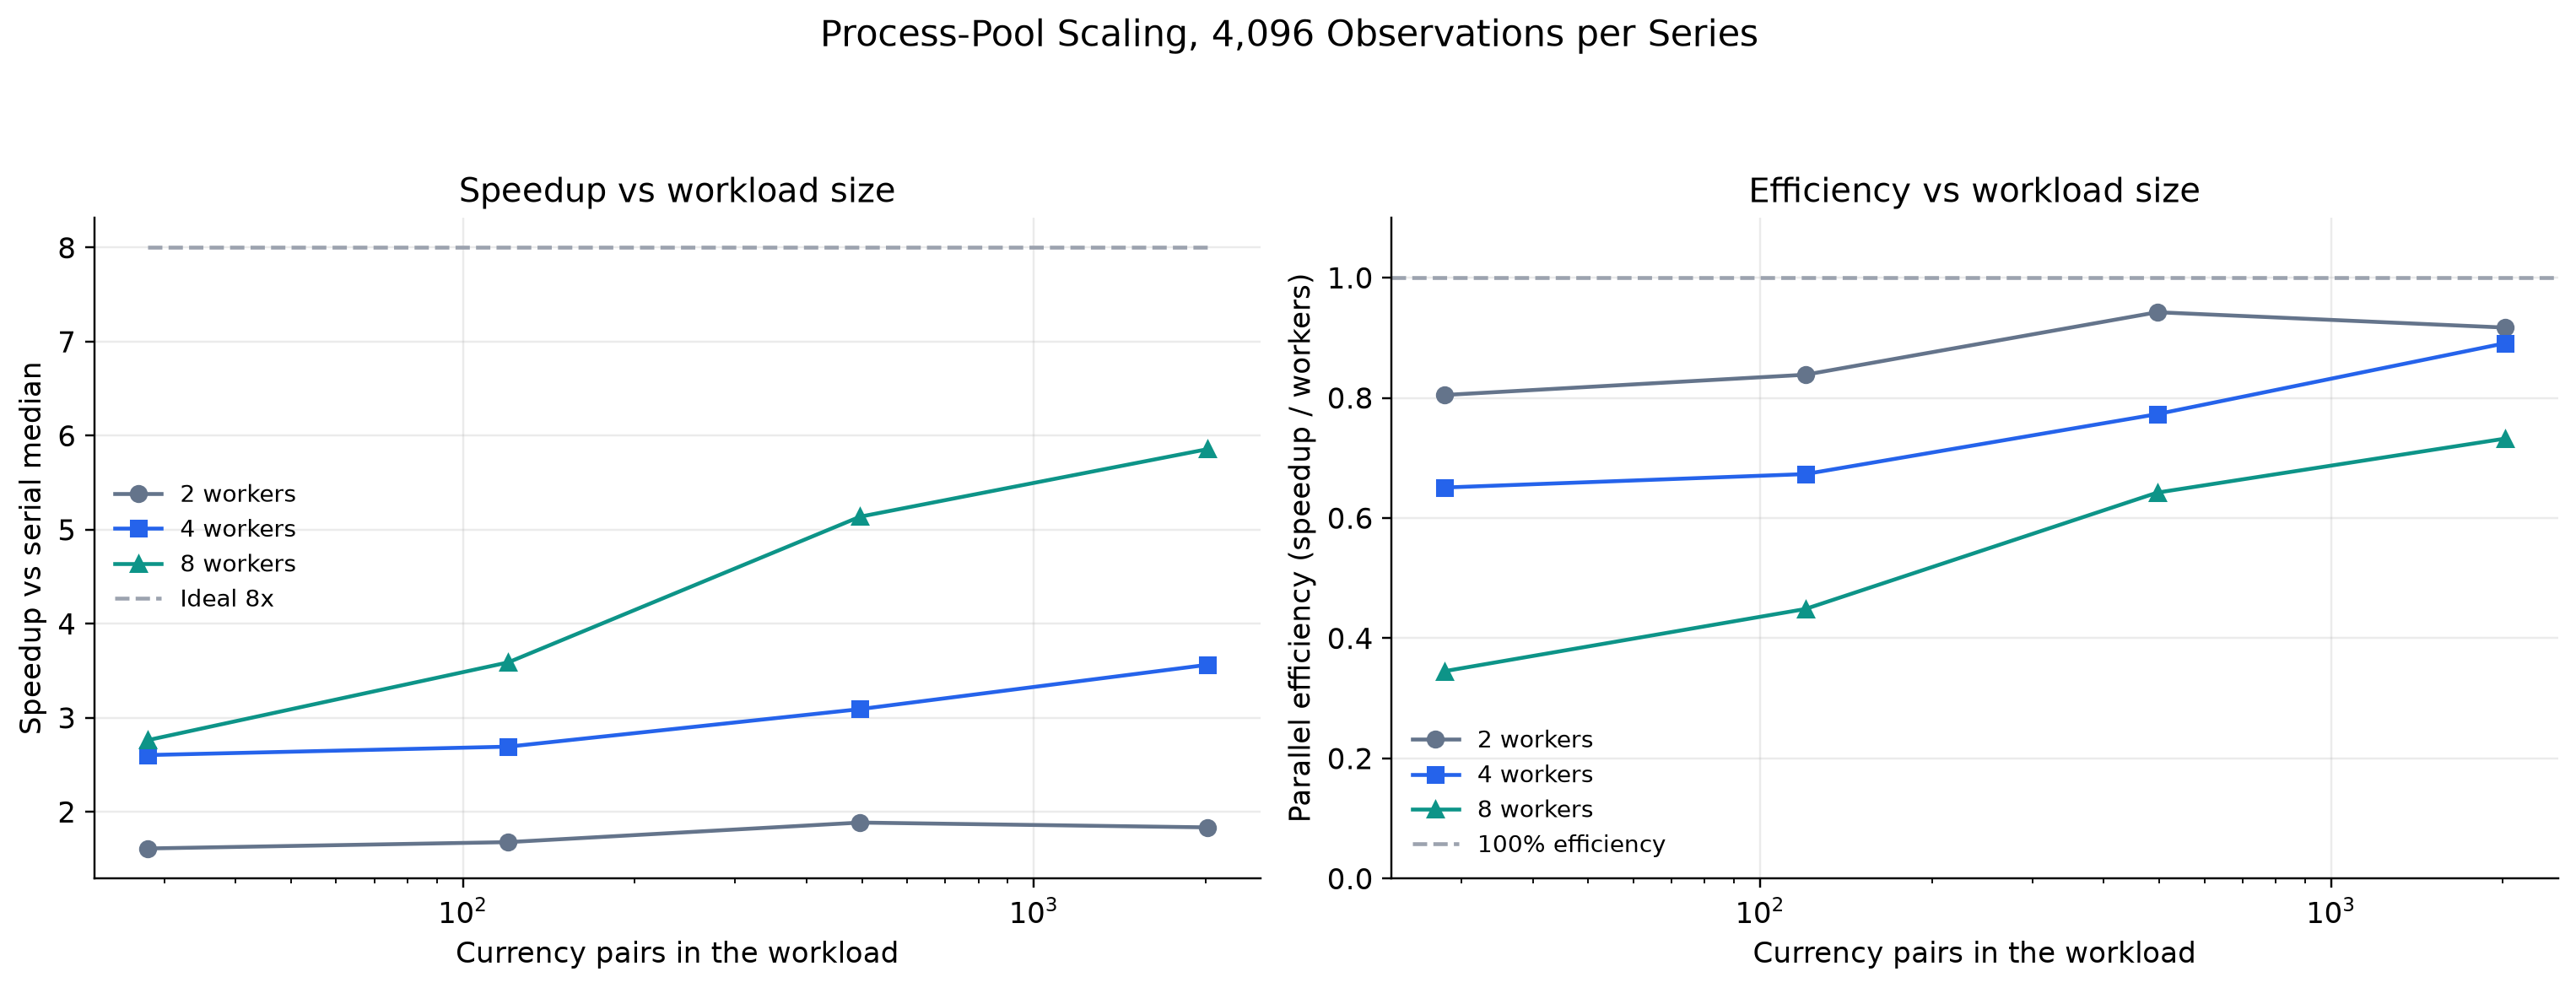
\includegraphics[width=0.9\textwidth]{figures/fig_scaling.png}
\caption{Speedup and parallel efficiency versus workload size for the process pool. The workload grows from 28 to 2,016 pairs at 4,096 observations; each point is the median of five repetitions.}
\label{fig:scaling}
\end{figure*}

\begin{figure}[t]
\centering
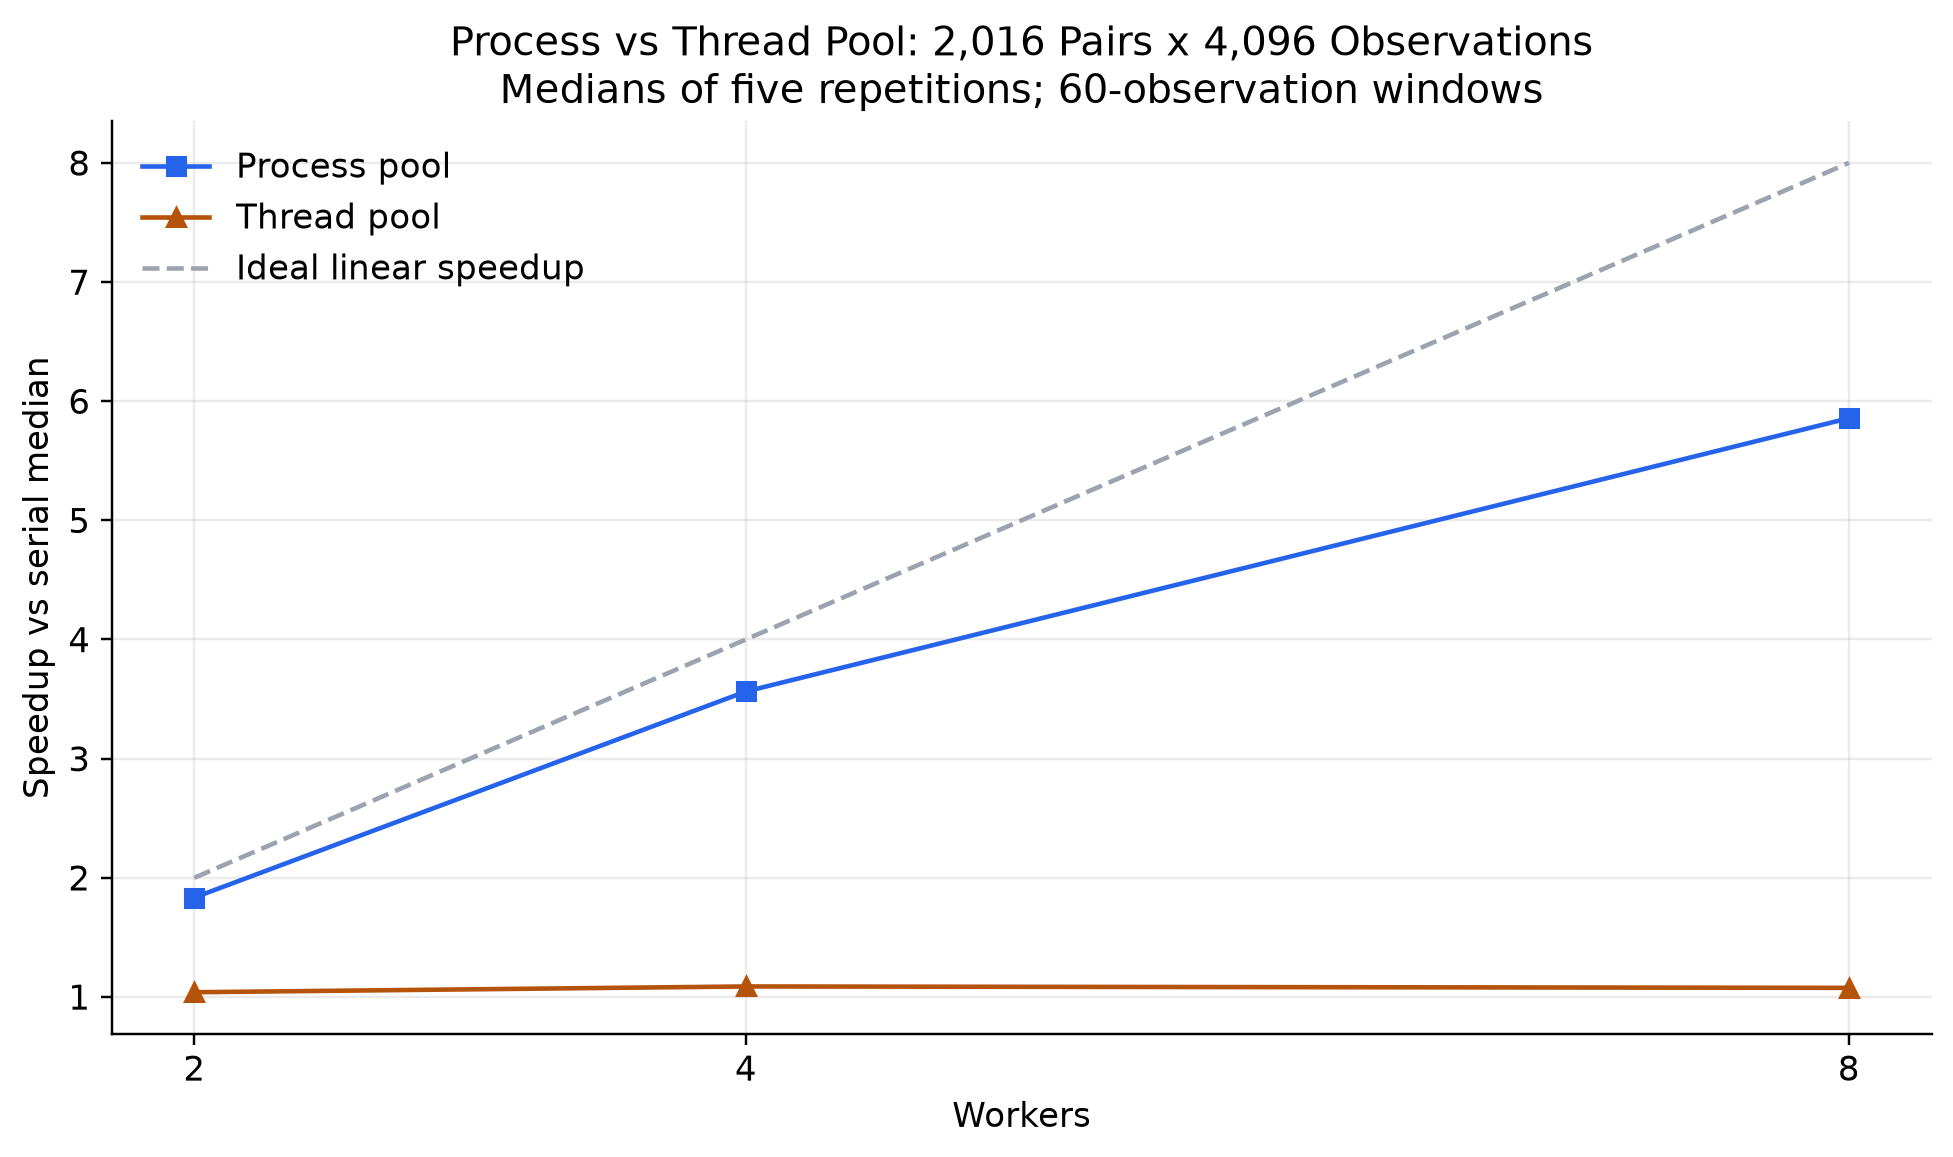
\includegraphics[width=\columnwidth]{figures/fig_threads.png}
\caption{Process versus thread pool at 2,016 pairs. The dashed line is ideal linear speedup; the thread pool stays close to 1$\times$.}
\label{fig:threads}
\end{figure}

% --------------------------------------------------------------------------
\section{Final Results}
\label{sec:results}

\subsection{What the data show}
The eight currencies do not share a common volatility level, and their correlation structure is not a single stable object. JPY has the highest full-period daily volatility (0.642\%), CHF the lowest (0.463\%), but CHF's extreme days dominate the tail: $-15.55\%$ on 2015-01-15 and $+8.00\%$ on 2011-09-06. The 60-observation volatility peak for CHF is 2.108\%, more than four times its full-period value, while JPY's peak is 1.256\%. This is the clearest example in the data of why a standard deviation and a tail statistic should be reported together.

The correlation results have a similar structure. USD--HKD is almost deterministic ($r = 0.9966$), and the CNY--USD--HKD group is strong (0.91). AUD--CAD is moderate (0.6134), while CHF--AUD is weak (0.1064). All 28 full-period correlations are positive, which is consistent with the common euro base. The rolling correlations show that the full-period values hide substantial time variation: JPY--AUD ranges from $-0.6009$ to 0.8077, and USD--JPY has the largest rolling standard deviation (0.2723). A reader who only saw the full-period matrix would miss both facts.

The cluster analysis summarises the same structure without adding a causal claim. USD and HKD merge first; CNY joins next; AUD and CAD form a pair; JPY joins the CNY--USD--HKD group; GBP joins AUD--CAD; CHF joins last. The two-, three- and four-cluster cuts are nested and exploratory. The bootstrap and the outlier check support the ranking: the Spearman correlation between the baseline and outlier-excluded vectors is 0.9956, and USD--HKD has a narrow interval [0.9948, 0.9977]. The weak pairs have wide intervals, which is the honest result for a 16-year sample with overlapping windows.

\subsection{Candidate interpretations}
Two observations invite a conjecture, which we keep separate from the descriptive results. The CHF move on 2015-01-15 coincides with the SNB's discontinuation of the EUR/CHF floor \cite{snb2015}; a policy-risk repricing is a plausible reading, but the daily data cannot identify the intraday mechanism or the counterfactual. The opposite GBP and JPY moves on 2016-06-24 coincide with the Brexit result \cite{ec2016}; a sterling repricing and a safe-haven flow are plausible, but we do not test that channel. The March 2020 cluster is consistent with a common global shock around the WHO pandemic declaration \cite{who2020}, with the same caveat. These are conjectures, not causal estimates; an event study with intraday data would be the next step.

\subsection{What the implementation shows}
The parallel results separate two questions that are often conflated: whether a pool can be faster at all, and whether it is faster at this workload. On the 28-pair task, a fresh pool is about 55 times slower than serial, and even a reused pool without batching does not beat serial. Batching at four workers reaches 1.64$\times$, but the absolute gain is about 7 ms and excludes the 0.9--1.0 s setup. For a single invocation of this analysis, serial execution is the right choice. The pool only becomes interesting when the workload is repeated or larger.

The scaling experiment shows where the crossover happens. At 2,016 pairs the eight-worker pool reaches 5.86$\times$ and 73\% efficiency; the thread pool remains near 1.08$\times$. The chunksize sweep shows that the gain is not automatic: a single chunk per workload is slower than serial, and the best chunk size depends on the worker count. The practical lesson is to batch, to broadcast worker-local data rather than re-pickling it per task, and to measure the setup cost before claiming an end-to-end speedup.

\subsection{Practical implications}
The data findings have a practical reading for currency-risk monitoring. A review that treats USD and HKD as separate exposures would overstate diversification: the pair moves almost as one series, and its rolling correlation never falls below 0.9163 in this sample. The weak CHF--AUD correlation (0.1064) is not a licence to assume independence; its bootstrap interval is wide, and the full-period value hides time variation. The JPY--AUD range from $-0.60$ to 0.81 is the clearest warning against a static correlation matrix: a limit calibrated on the full-period average would misstate the relationship in both directions. The cluster map is a coarse grouping for exposure review, not a trading rule. On the computing side, a single 20 ms analysis should stay serial; a repeated or larger pipeline should reuse a prepared pool, batch tasks and measure setup costs before claiming an end-to-end speedup.

\subsection{Against the brief}
The Open Project brief asks for data collection with a documented source, preprocessing and visualisation, an advanced analysis with findings, a parallel implementation with correctness checks and performance comparison, and a conclusion with limitations. The report covers each item. Success is judged on evidence quality, reproducibility and a defensible parallel analysis, not on a leaderboard rank. We therefore make no ranking claim. We do claim that the reported numbers are reproducible from the public data and the included scripts, and that the negative results (fresh pool, unbatched pool, threads) are reported rather than hidden.

The main limitation is scope. Eight currencies, one 16-year sample and daily reference rates cannot support a general theory of currency co-movement. The clustering is exploratory, the bootstrap is approximate, and the parallel measurements come from one machine. The synthetic scaling data are a benchmark device. These limits are not defects to be argued away; they define what the evidence can support.

% --------------------------------------------------------------------------
\section{AI Tool Usage Statement}
\label{sec:ai}

% NOTE: Complete this statement truthfully. The course permits AI use for
% debugging, API queries, idea discussion and language polishing, but requires
% disclosure and prohibits submitting AI-generated complete work verbatim.
% Replace the bracketed items with the tools and division of work actually used.

AI assistants were used for code debugging and refactoring, documentation drafting, and language editing. ChatGPT and DeepSeek were the tools used. The data-processing and analysis steps, the main issues raised during the work, and the solutions adopted were set and verified by the group. The tools were not used to produce the final submission verbatim. The authors specified the research questions, selected the data, designed the analyses, ran the pipeline, checked the reported numbers against the saved CSV files and figures, and rewrote the text where necessary. The parallel benchmark design, the sensitivity checks and the interpretation of the results were reviewed by all authors.

The core implementation was completed by the group: the cleaning script, the return and rolling-window calculations, the correlation and clustering analyses, the process-pool benchmark, the scaling experiment and the figure-generation pipeline. AI assistance was used to suggest refactorings, catch edge cases such as the date-format mismatch, and improve the clarity of the prose. All suggestions were tested before they were kept; the archived outputs in the repository document the runs that were superseded.

% --------------------------------------------------------------------------
\section{Discussion and Reflection}
\label{sec:discussion}

The parts that worked are easy to name. Log changes, a documented quote direction, and a sample-standard-deviation convention removed a large class of silent errors. The \texttt{allclose} check between serial and parallel results made the parallel work trustworthy; without it, a speedup number would be meaningless. Forcing every worker to start before timing exposed a bug in the first scaling script, where the executor was still starting workers during the measured runs. Batching and worker-local data turned a flat or negative result into a measurable gain.

The parts that did not work are equally useful. A fresh pool is not a sensible default for a 20 ms workload. A reused pool without batching is not either. Threads do not scale here, which is consistent with the GIL but is still worth measuring rather than assuming. The 8-worker efficiency is 73\%, not 100\%, and the Amdahl check suggests that the shortfall is not a fixed serial section but overhead that grows with the worker count. The initial note also contained a hard-coded claim that pool reuse always helps; the data did not support it, and the note was rewritten to follow the measurements.

The limitations are mostly about scope and measurement. The data are daily reference rates, so intraday dynamics and transaction costs are out of reach. The common euro base means that a positive correlation is not a bilateral statement. The bootstrap blocks preserve short-range dependence but not the exact overlap structure of rolling windows. The benchmark is one machine, one Python build and one session; the medians are not confidence intervals, and a different machine would change the absolute times. The synthetic scaling series are useful for varying workload size but are not evidence about currency markets.

Future work could move in three directions. A higher-frequency dataset would allow event studies around the 2015 and 2016 dates and a proper intraday volatility analysis. A factor decomposition could separate the common euro movement from bilateral components, which would make the correlation matrix easier to interpret. On the computing side, a Spark or Hadoop comparison at a much larger scale would test whether the process-pool conclusions extend beyond a single machine; at the present data size, the start-up and coordination costs of a distributed framework would dominate.

\subsection{Conclusion}
The four questions have short answers. Volatility is heterogeneous: JPY has the highest full-period level, CHF the lowest, and CHF's tail is the largest. Correlation is not a single stable number: USD--HKD is almost deterministic, CHF--AUD is weak, and pairs such as JPY--AUD change sign. Clustering summarises the full-period structure but is exploratory, and its ranking survives the window and outlier checks. Parallelism is not automatically beneficial: a fresh pool loses badly on 28 pairs, batching recovers 1.64$\times$, and the process pool reaches 5.86$\times$ at 2,016 pairs while threads stay near 1$\times$.

The pros of the approach are a public and reproducible data source, explicit quote and window conventions, numerical checks that make the parallel claim meaningful, and a scaling study that reports the negative cases. The cons are equally clear: the analysis is descriptive, the cross-section is small, the observations are daily reference rates, the rolling windows overlap, and the benchmarks come from one machine. The synthetic scaling data are a benchmark device, not market evidence. We would rather state these limits than hide them behind a single headline number.

% --------------------------------------------------------------------------
\section{Reproducibility}
\label{sec:reproducibility}

The pipeline was run with Python 3.11.9, NumPy 2.4.6 \cite{harris2020}, pandas 3.1.1 \cite{mckinney2010}, Matplotlib 3.11.2 \cite{hunter2007} and SciPy 1.17.1 \cite{virtanen2020} on Windows with 16 logical CPUs. Process pools use the \texttt{spawn} start method. The bootstrap uses seed 20261122 and 1,000 replicates; the scaling experiment uses the same seed and a deterministic factor model. The descriptive analyses have no random component.

The repository is organised around a fixed run order: cleaning, returns, descriptive statistics, plots, correlation and clustering, rolling volatility and correlation, monthly and extreme analyses, robustness checks, and the parallel benchmarks. The exact commands are listed in the README. After the benchmarks, \texttt{python data/regenerate\_figures.py} rebuilds all 22 figures from code; the benchmark figures are redrawn from the frozen CSV summaries, so the figures can be regenerated without re-measuring the timings. This separation matters because timing medians drift with machine load.

The ECB file is a snapshot that contains observations through 2026-11-20. Re-downloading later will add rows; the cleaning script filters to the project period, so the analysis remains comparable, but the last observation and the file hash will differ. The environment CSVs record the interpreter, library versions and CPU count for the benchmark runs. Absolute times should be compared within a run, not across machines.

Code and supporting material: \url{https://github.com/YifanHuang-if/CS4480-Project}.

% --------------------------------------------------------------------------
\section{Relative Contribution}
\label{sec:contribution}

Table~\ref{tab:contributions} lists each member's actual productive hours.

\begin{table}[t]
\caption{Team contribution breakdown (actual productive hours).}
\label{tab:contributions}
\centering
\small
\renewcommand{\arraystretch}{1.25}
\begin{tabular}{l|c}
\hline
\textbf{Member} & \textbf{Total Hours} \\
\hline
Wu Kunze & 12 \\
\hline
Feng Xinyi & 10 \\
\hline
Huang Yifan & 11 \\
\hline
\textbf{Team Total} & \textbf{33} \\
\hline
\end{tabular}
\end{table}

% --------------------------------------------------------------------------
\begin{thebibliography}{10}

\bibitem{ecb}
European Central Bank, ``Euro foreign exchange reference rates,'' 2026. [Online]. Available: \url{https://www.ecb.europa.eu/stats/policy_and_exchange_rates/euro_reference_exchange_rates/html/index.en.html}

\bibitem{snb2015}
T.~J. Jordan, ``The rationale for discontinuing the minimum exchange rate and lowering interest rates,'' Swiss National Bank, Zurich, Switzerland, Jan.~2015. [Online]. Available: \url{https://www.bis.org/speeches/20150116-rationale-discontinuing-minimum-exchange-rate-and-lowering-interest-rates}

\bibitem{ec2016}
Electoral Commission, ``Official result of the EU referendum is declared by the Electoral Commission in Manchester,'' Jun.~2016. [Online]. Available: \url{https://www.electoralcommission.org.uk/media-centre/official-result-eu-referendum-declared-electoral-commission-manchester}

\bibitem{who2020}
World Health Organization, ``WHO Director-General's opening remarks at the media briefing on COVID-19 --- 11 March 2020,'' Mar.~2020. [Online]. Available: \url{https://www.who.int/news-room/speeches/item/who-director-general-s-opening-remarks-at-the-media-briefing-on-covid-19---11-march-2020}

\bibitem{harris2020}
C.~R. Harris \emph{et al.}, ``Array programming with NumPy,'' \emph{Nature}, vol.~585, pp.~357--362, 2020.

\bibitem{mckinney2010}
W.~McKinney, ``Data structures for statistical computing in Python,'' in \emph{Proc. 9th Python in Science Conf.}, 2010, pp.~56--61.

\bibitem{virtanen2020}
P.~Virtanen \emph{et al.}, ``SciPy 1.0: fundamental algorithms for scientific computing in Python,'' \emph{Nature Methods}, vol.~17, pp.~261--272, 2020.

\bibitem{hunter2007}
J.~D. Hunter, ``Matplotlib: A 2D graphics environment,'' \emph{Computing in Science \& Engineering}, vol.~9, no.~3, pp.~90--95, 2007.

\bibitem{amdahl1967}
G.~M. Amdahl, ``Validity of the single processor approach to achieving large scale computing capabilities,'' in \emph{Proc. AFIPS Spring Joint Computer Conference}, 1967, pp.~483--485.

\bibitem{python}
Python Software Foundation, ``multiprocessing --- Process-based parallelism,'' Python 3.11 documentation. [Online]. Available: \url{https://docs.python.org/3.11/library/multiprocessing.html}

\end{thebibliography}

\end{document}
